%-----------------------------------------------------------------------------%
\chapter{HASIL PENELITIAN DAN PEMBAHASAN}
%-----------------------------------------------------------------------------%

%
\vspace{4.5pt}
\begin{flushleft}
    \begin{justify}
        \section{Hasil Penelitian}
        \subsection{Hasil Observasi}
        Peneliti mengamati kebutuhan sensor dan kontrol yang sering diaplikasikan pada lahan secara umum untuk kebutuhan pembuatan aplikasi KEBUNQ. Didapat data sebagai berikut.\\
        \subsubsection{Sensor} 
        Beberapa sensor yang akan digunakan pada lahan pertanian yang perlu dicantumkan ke aplikasi KEBUNQ adalah sebagai berikut:
        \begin{enumerate}
            \item Sensor suhu untuk mengukur nilai suhu ruangan
            \item Sensor \emph{humidity} untuk mengukur kelembapan
            \item Sensor intensitas cahaya untuk mengukur intensitas cahaya
            \item Sensor suhu tanah
            \item Sensor \emph{humidity} tanah untuk mengukur kelebapan tanah
            \item Sensor pH tanah untuk mengukur kandungan pH yang terdapat di tanah
            \item Sensor suhu air untuk mengukur suhu pada air
            \item Sensor TDS (ppm meter) untuk mengukur kadar TDS (\emph{Total Dissolve Solid}) dalam air.
            \item Sensor pH air untuk mengukur kandungan pH yang terdapat di air\\
        \end{enumerate}
        \subsubsection{Kontrol}
        Berikut beberapa kontrol yang biasa digunakan pada lahan pertanian yang perlu dicantumkan ke aplikasi KEBUNQ :
        \begin{enumerate}
            \item \emph{Mist} 
            \\Digunakan untuk melakukan pengabutan, ketika menyala akan mengeluarkan kabut air. 
            Berikut ilustrasi \emph{mist} dapat dilihat pada Gambar 4.1.\\
            \begin{figure}[ht]
                \centering
                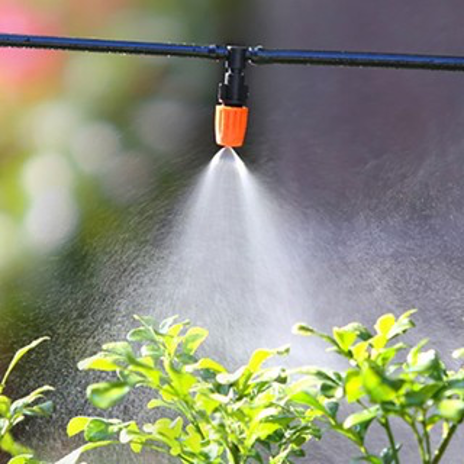
\includegraphics[width=8cm]{images/bab 4/gambar_mist.png}
                \caption{Ilustrasi \textit{Mist}}
            \end{figure}
            \item \emph{Sprinkler} 
            \\Digunakan untuk melakukan penyiraman, ketika menyala \emph{sprinkler} akan menyemprotkan air.
            Berikut ilustrasi \emph{sprinkler} dapat dilihat pada Gambar 4.2.
            \begin{figure}[ht]
                \centering
                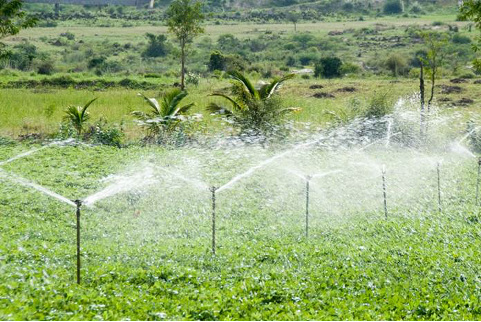
\includegraphics[width=10cm]{images/bab 4/gambar_sprinkler.png}
                \caption{Ilustrasi \textit{Sprinkler}}
            \end{figure}
            \item \emph{Fan} 
            \\Digunakan untuk memberikan hembusan angin, ketika menyala \emph{fan} akan meniupkan angin.
            Berikut ilustrasi \emph{fan} dapat dilihat pada Gambar 4.3.\\\\
            \begin{figure}[ht]
                \centering
                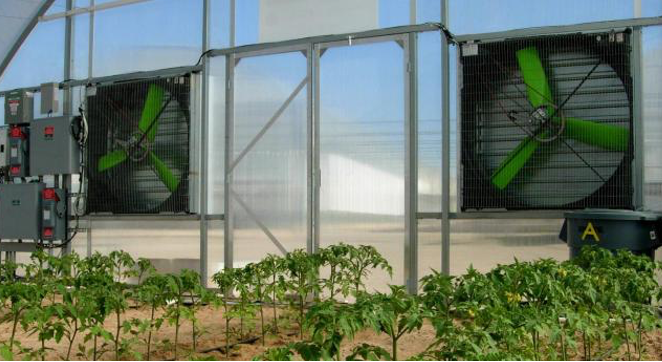
\includegraphics[width=11cm]{images/bab 4/gambar_fan.png}
                \caption{Ilustrasi \textit{Fan}}
            \end{figure}
            \item \emph{Valve} 
            \\Digunakan untuk membuka alur aliran air selayaknya keran air, ketika menyala \emph{valve} akan membuka aliran air pada selang.
            Berikut bentuk \emph{valve} dapat dilihat pada Gambar 4.4.
            \begin{figure}[ht]
                \centering
                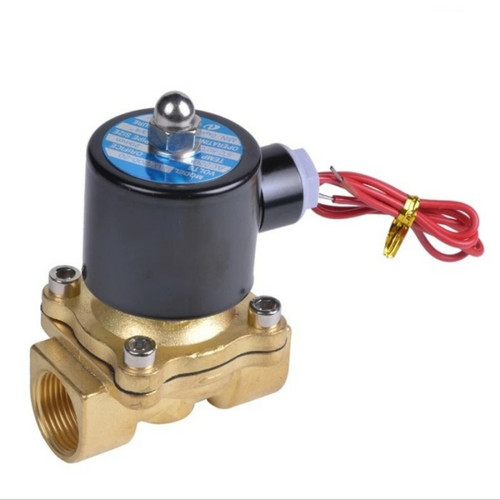
\includegraphics[width=7cm]{images/bab 4/gambar_valve.jpeg}
                \caption{Bentuk \textit{Valve}}
            \end{figure}
            \item \emph{Drip} 
            \\Digunakan untuk melakukan pemupukan, ketika menyala \emph{drip} akan meneteskan air yang sudah disiapkan.
            Berikut ilustrasi \emph{drip} dapat dilihat pada Gambar 4.5.
            \vspace{4cm}
            \begin{figure}[ht]
                \centering
                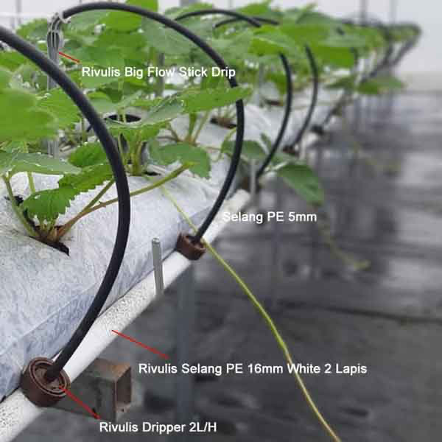
\includegraphics[width=7cm]{images/bab 4/gambar_drip.png}
                \caption{Ilustrasi \textit{Drip}}
            \end{figure}
            \item Pompa 
            \\Digunakan untuk membantu mengalirkan air, 
            ketika menyala pompa akan menghisap air dari sumber air yang tersedia.
            Berikut bentuk pompa dapat dilihat pada Gambar 4.6.
            \begin{figure}[ht]
                \centering
                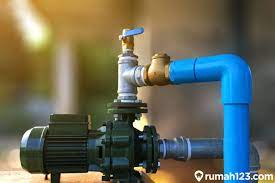
\includegraphics[width=10cm]{images/bab 4/gambar_pompa.jpeg}
                \caption{Pompa}
            \end{figure}
            \item Lainnya (\emph{Customize})\\
            Dibuat untuk menampung bentuk kontrol ketika terdapat kontrol selain yang tercantum pada poin 1 hingga 6.\\
        \end{enumerate}
        % \caption{Gambar Observasi}
        \subsection{Hasil Penerapan RAD}
        Sebelum masuk pada pembahasan per proses dalam RAD, berikut dicantumkan jadwal pengerjaan 
        sistem KEBUNQ secara menyeluruh dengan mengimplementasikan RAD.
        \begin{figure}[ht]
            \centering
            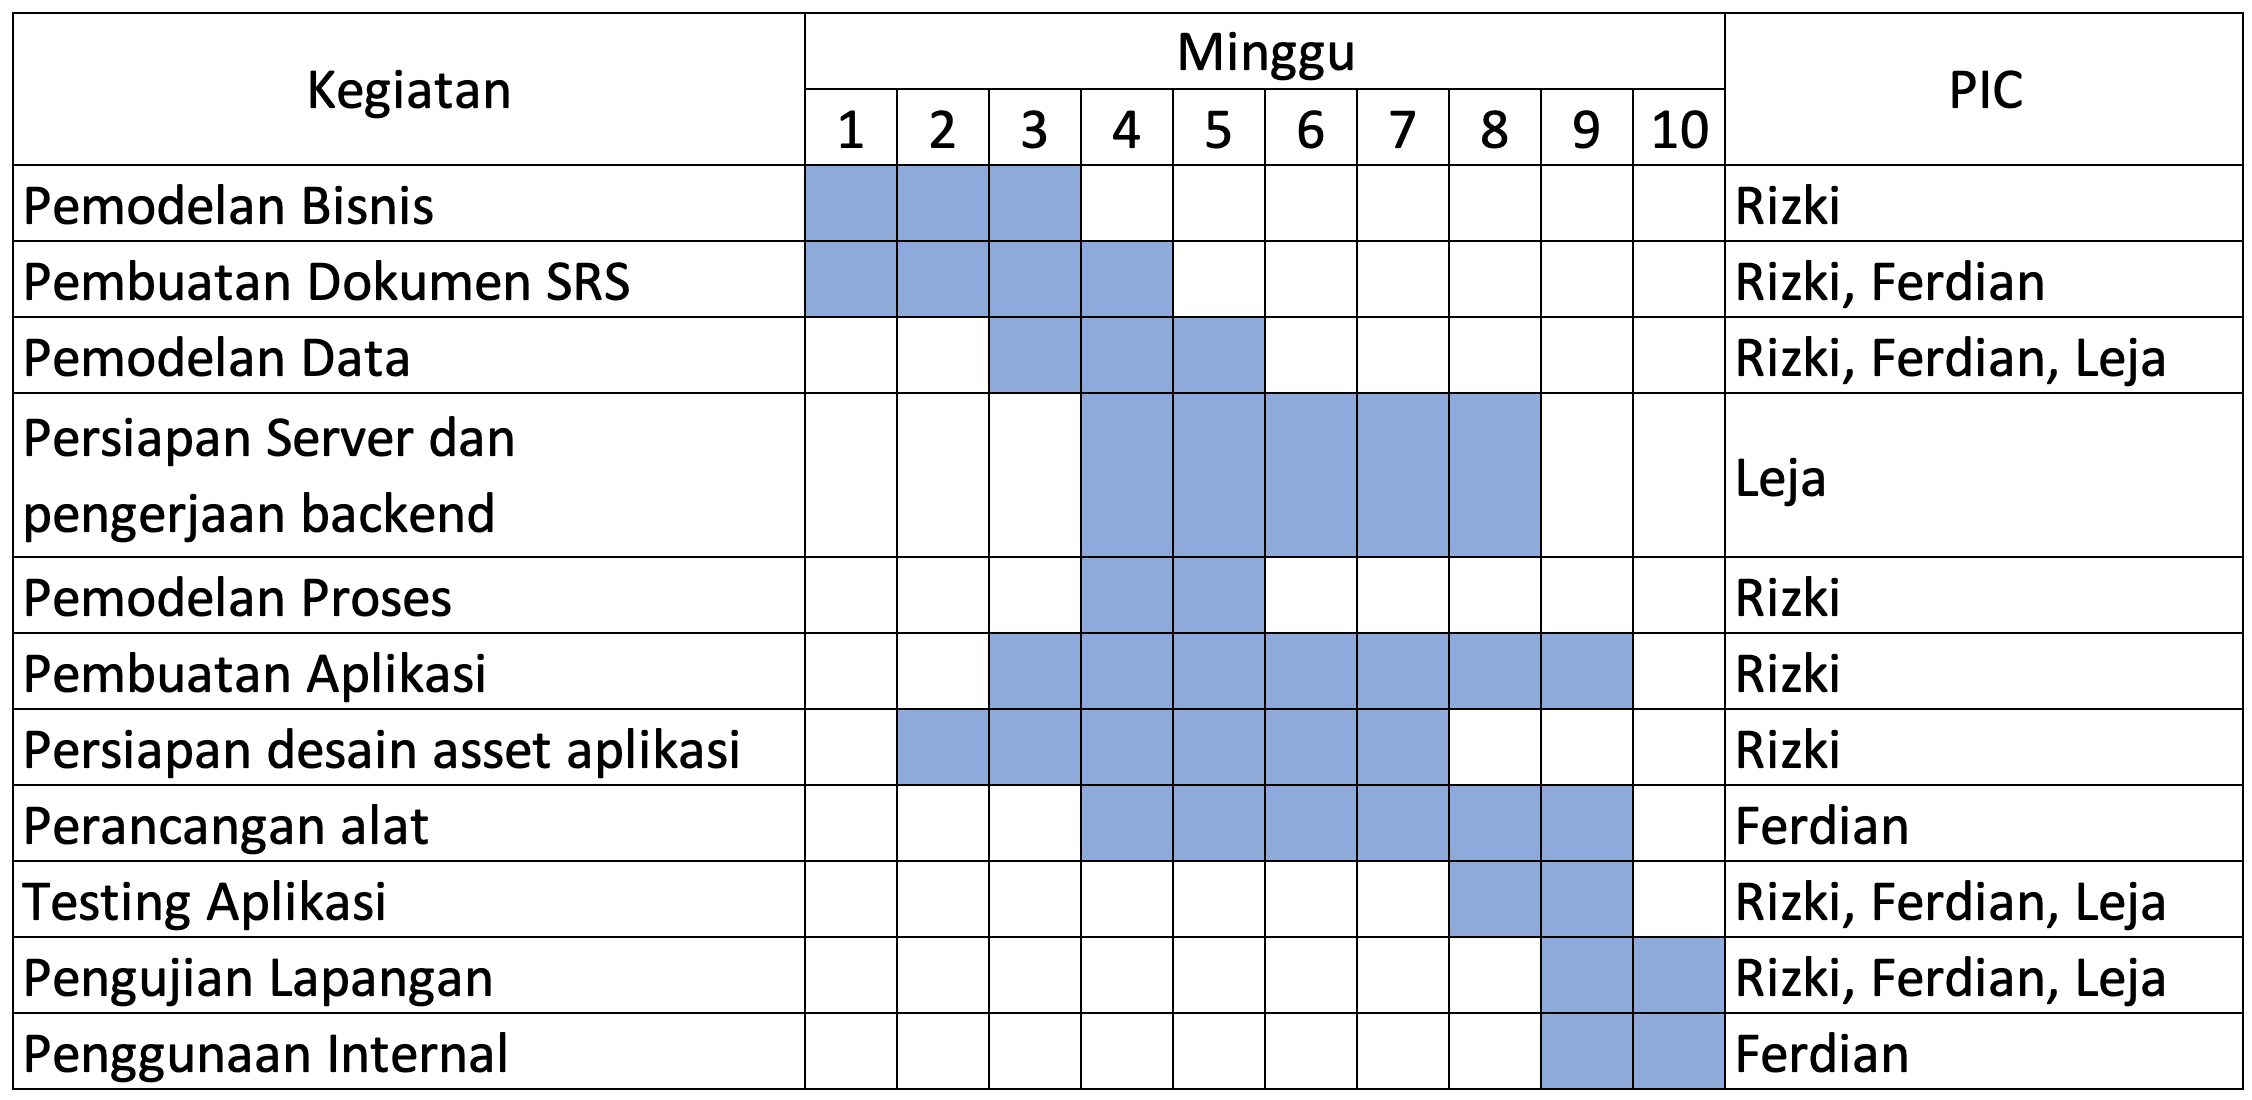
\includegraphics[width=14cm]{images/bab 4/gantt.png}
            \caption{Jadwal Pengerjaan}
        \end{figure}

        \noindent Pada Gambar 4.7 dapat dilihat bahwa beberapa pengerjaan dilakukan dengan cara bersamaan 
        dan paralel oleh anggota tim. Tedapat tiga bagian khusus yang pengerjaannya dibagi, yaitu persiapan server
        dan pengerjaan \emph{backend} yang dilakukan oleh anggota tim bernama Leja, pembuatan aplikasi yang dikerjakan oleh Rizki (peneliti), dan pengerjaan
        perancangan alat yang dilakukan oleh anggota tim bernama Ferdian. Pengerjaan proyek ini memiliki \emph{stakeholder} dari pihak BPP Lampung. 
        
        Kemudian berikut hasil yang didapatkan dari setiap proses dalam pemngimplementasian RAD:\\
        \subsubsection{Pemodelan Bisnis}
        Berdasarkan hasil analisa ditentukan bahwa aplikasi KEBUNQ dirancang untuk satu jenis pengguna. Sehingga tidak terdapat level pengguna pada akses aplikasi.
        Berikut analisa kebutuhan pengguna
        \begin{enumerate}
            \item Pengguna harus melakukan login
            \item Pengguna dapat melihat daftar dan status nyala alat
            \item Pengguna dapat melihat detail alat yang terdiri dari data sensor dan kontrol yang tersedia
            \item Pengguna dapat melakukan kontrol pada alat yang dipilih
            \item Pengguna dapat melakukan setting automatis pada suatu kontrol yang tersedia mode automatisnya
        \end{enumerate}
       Dari proses pemodelan bisnis ini juga sekaligus dibuat SRS yang terdapat pada lampiran penelitian.\\
        \subsubsection{Pemodelan Data}
        \begin{figure}[ht]
            \centering
            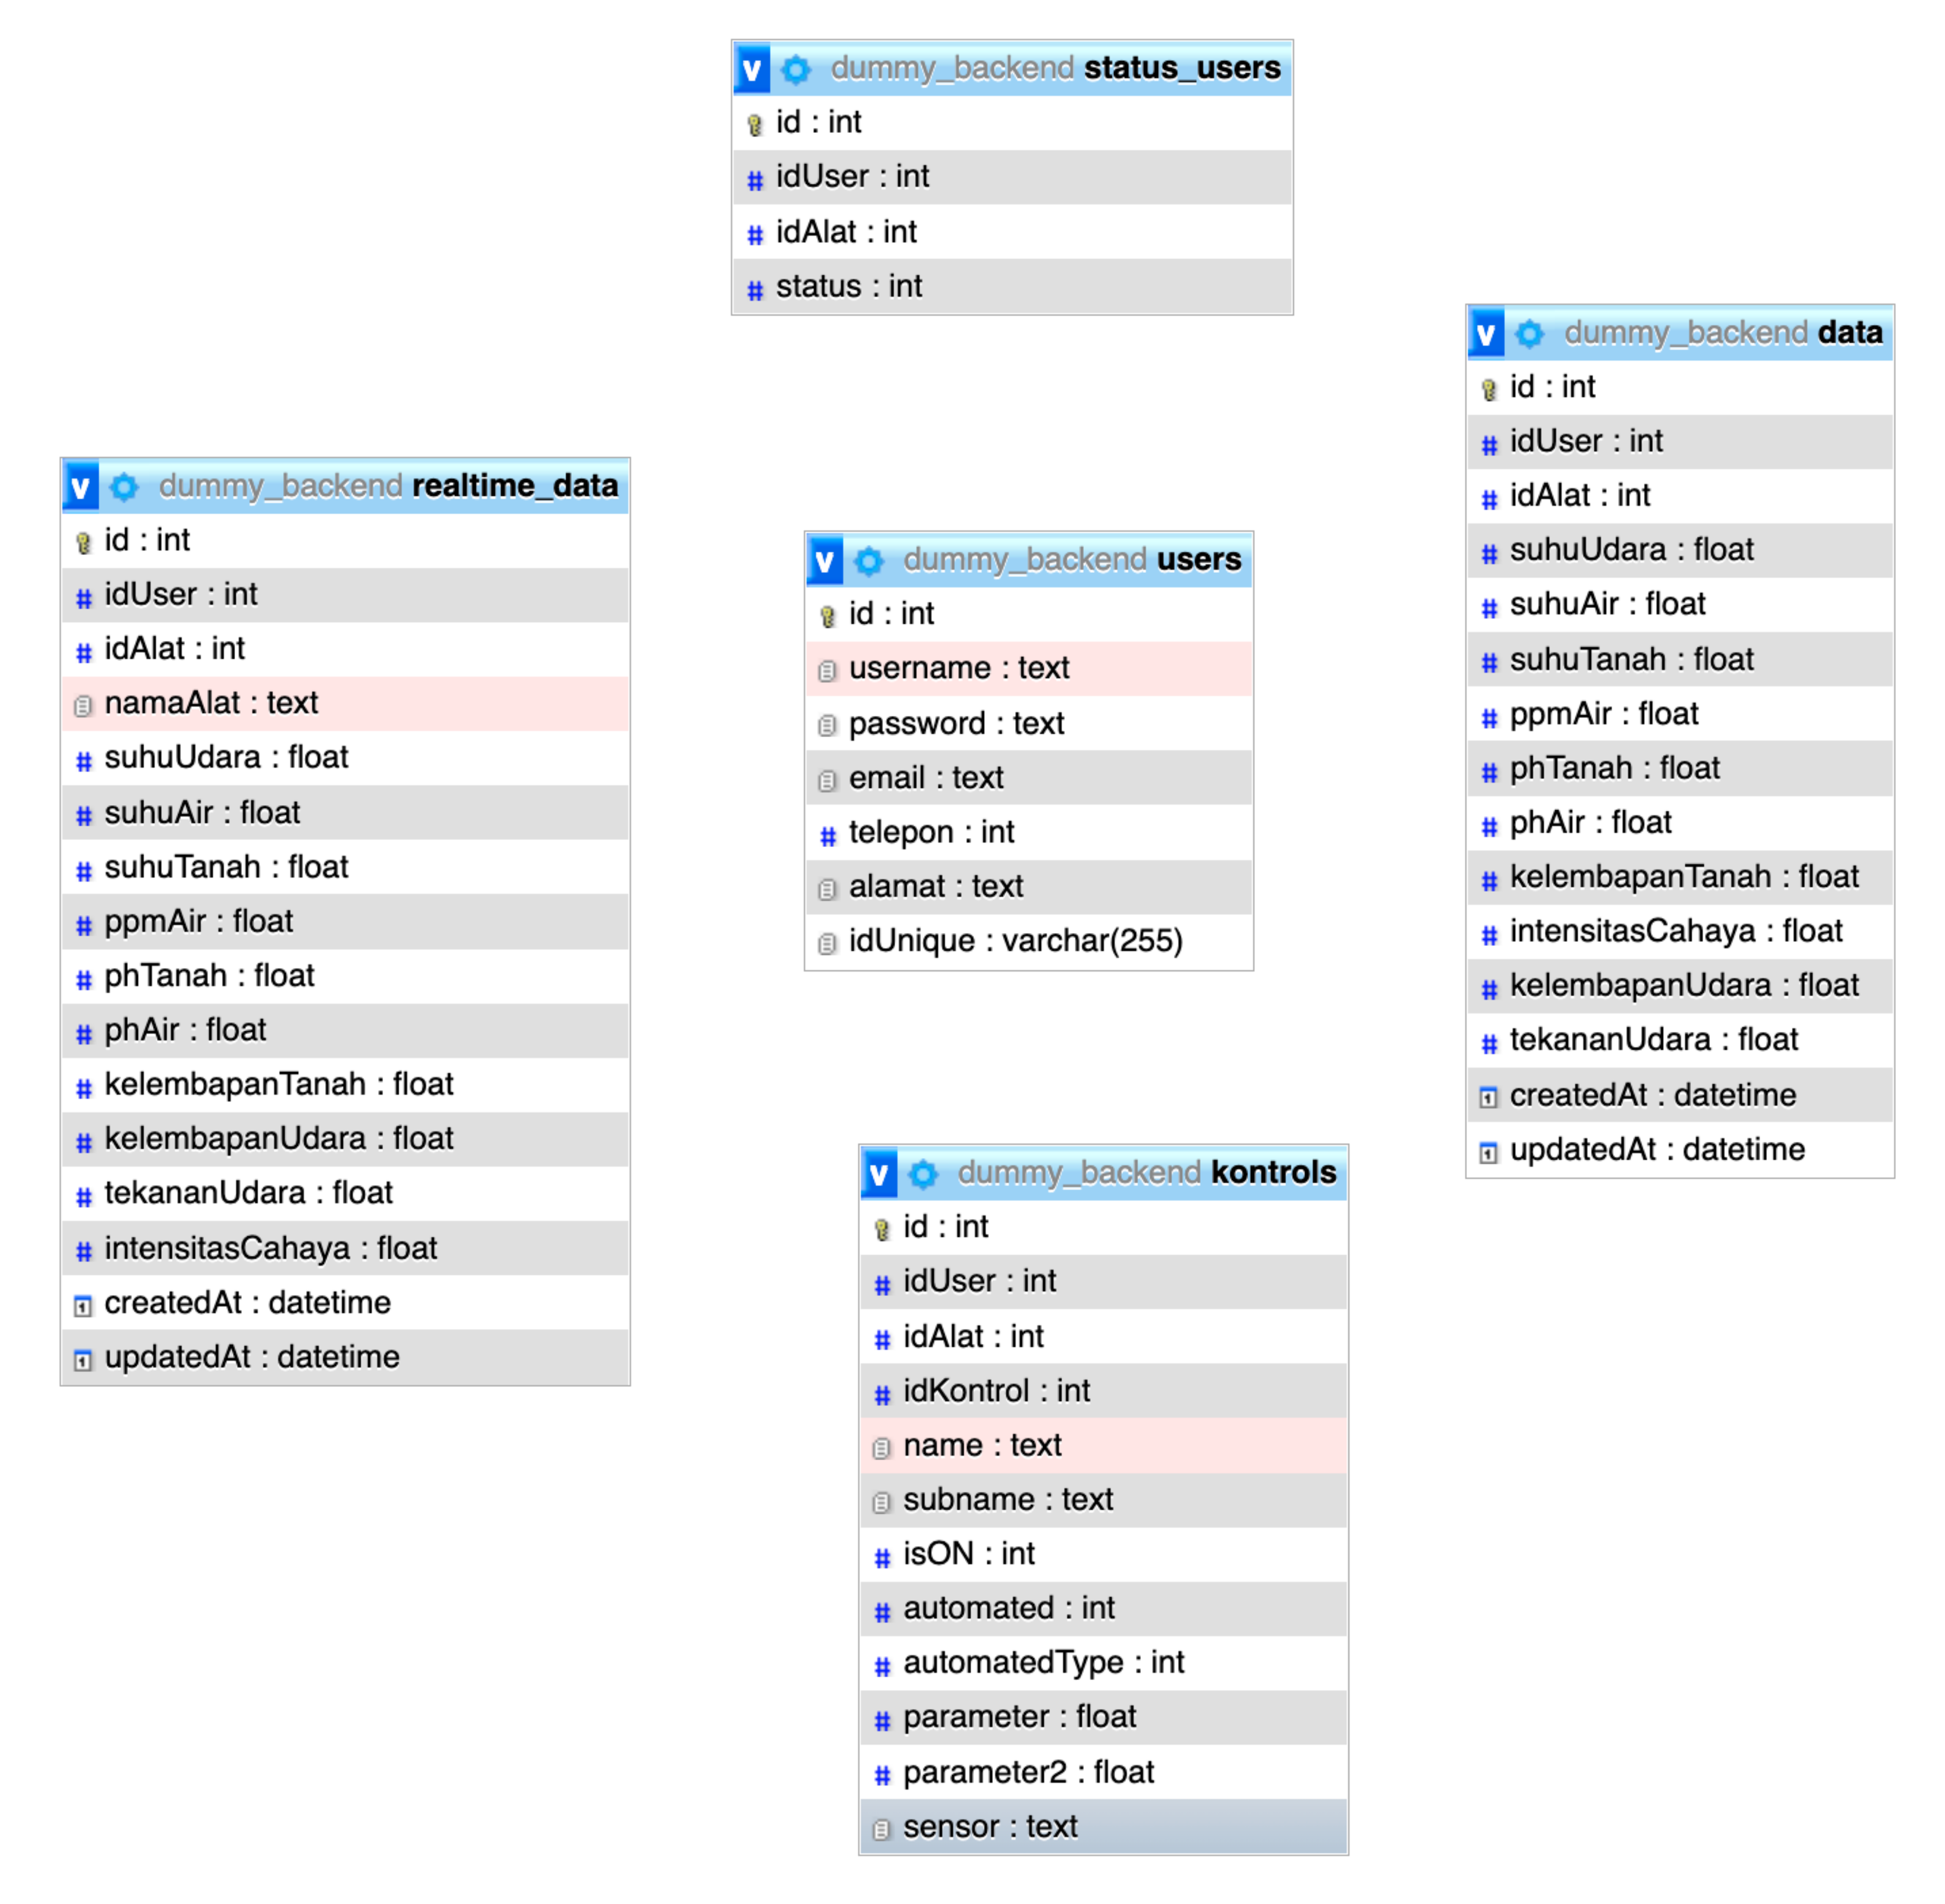
\includegraphics[width=12cm]{images/database.png}
            \caption{Skema Tabel \textit{Database}}
        \end{figure}
        \noindent Setelah dilakukan tahap pemodelan bisnis, maka didapatkan skema \emph{database} yang 
        dirancang seperti gambar 4.8 di atas. \emph{Database} terdiri dari lima tabel yaitu sebagai berikut:
        \begin{enumerate}
            \item Tabel data, digunakan untuk menyimpan data time series dari nilai sensor yang ada pada alat, 
            \item Tabel kontrols, digunakan untuk menyimpan dan mendefinisikan kontrol yang dimiliki, 
            \item Tabel realtime\_data, digunakan untuk menyimpan data realtime sensor dan kontrol,
            \item Tabel status\_users, digunakan untuk menyimpan status alat apakah \emph{online} atau \emph{offline},
            \item Tabel users, digunakan untuk menyimpan data user.
        \end{enumerate}
        Dapat dilihat juga bahwa tabel user berada di tengah dan memiliki relasi \emph{one to many} ke keempat tabel lain. Setelah skema \emph{database} difinalisasi, 
        maka dilakukan pembuatan \emph{Application Programming Interface} (API) dan konfigurasi server yang dalam bagian ini 
        pengerjaan bukan dilakukan oleh peneliti namun oleh anggota lain dalam proyek. 
        Sehingga akhirnya didapat beberapa API (\emph{dummy}) sebagai berikut dengan \emph{endpoint} yang dirahasiakan demi keamanan aplikasi :
            \begin{itemize}
                \item API login\\
                http://47.89.212.89/dummyBackend/(\emph{endpoint})
                \\Digunakan untuk melakukan \emph{post login}.
                \item API \emph{Summary Data} dari pengguna\\
                http://47.89.212.89/dummyBackend/data/(\emph{endpoint})\\
                Merupakan data rangkuman dari keseluruhan data yang dimiliki seorang pengguna. 
                Berikut contoh tampilan API
                \emph{Summary Data} dari pengguna dapat dilihat pada Gambar 4.9.
                \begin{figure}[ht]
                    \centering
                    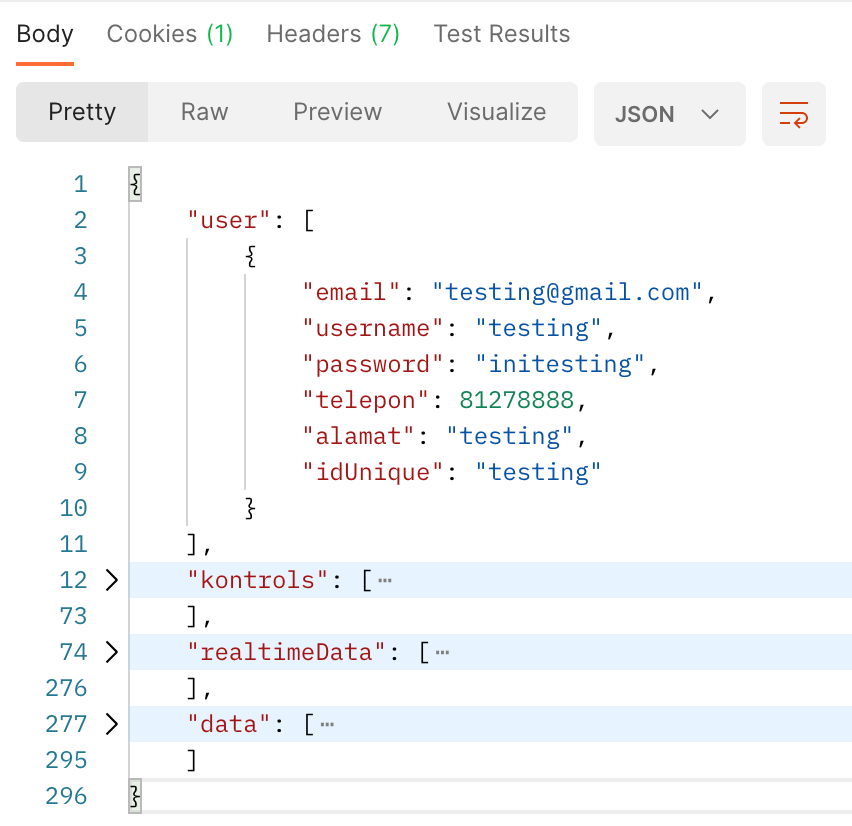
\includegraphics[width=9cm]{images/bab 4/api/summary.png}
                    \caption{API \textit{Summary} Pengguna}
                \end{figure}
                \item API data \emph{realtime}\\
                http://47.89.212.89/dummyBackend/data/mobile/(\emph{endpoint})\\
                Merupakan API yang menyediakan bagian data \emph{realtime} dari sebuah alat yang dimiliki pengguna.
                Berikut contoh tampilan API data
                \emph{realtime} dapat dilihat pada Gambar 4.10.
                \begin{figure}[ht]
                    \centering
                    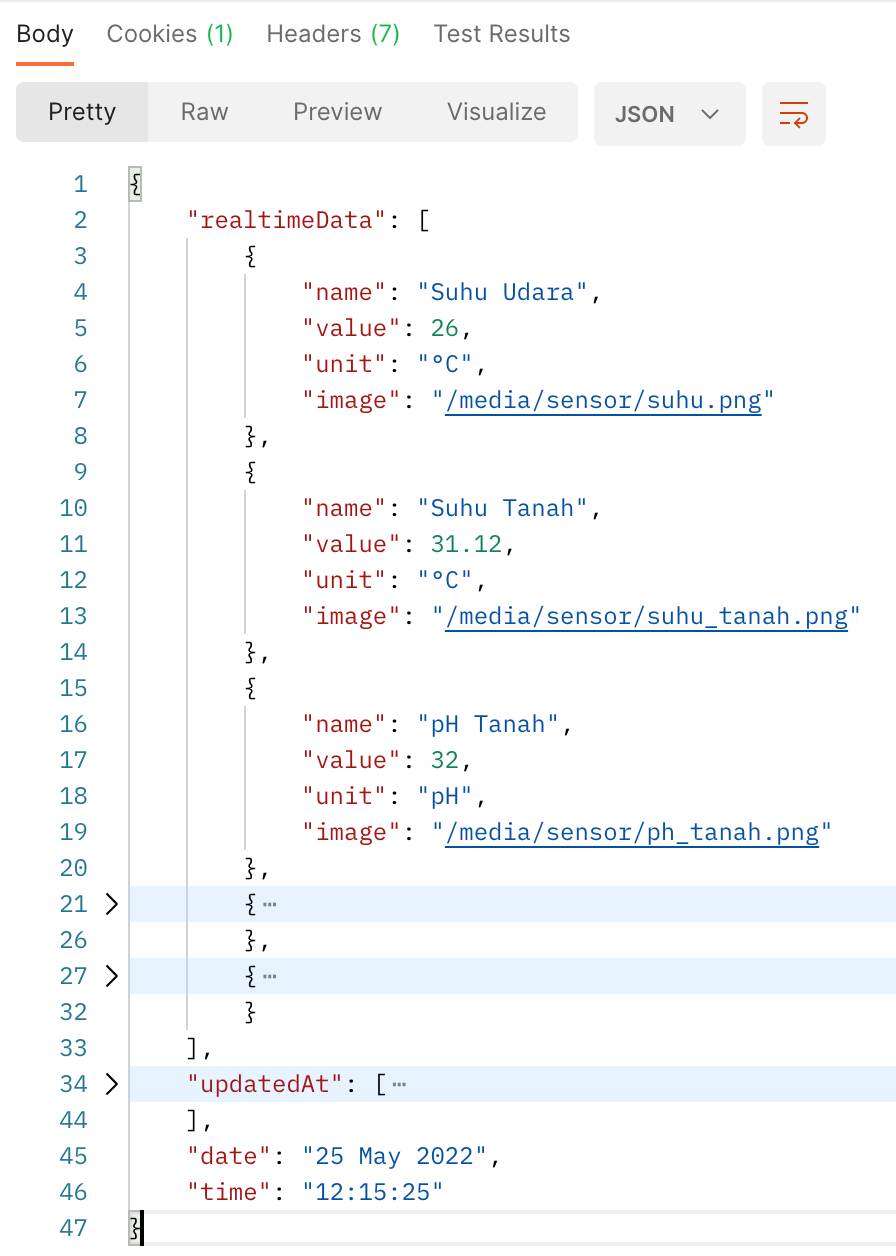
\includegraphics[width=9cm]{images/bab 4/api/realtime.png}
                    \caption{API Data \textit{Realtime}}
                \end{figure}
                \item API data kontrol\\
                http://47.89.212.89/dummyBackend/kontrol/(\emph{endpoint})\\
                Merupakan API yang berisikan data kontrol dari sebuah alat yang dimiliki pengguna.
                Berikut contoh tampilan API data kontrol
                dapat dilihat pada Gambar 4.11.
                \vspace{8cm}
                \begin{figure}[ht]
                    \centering
                    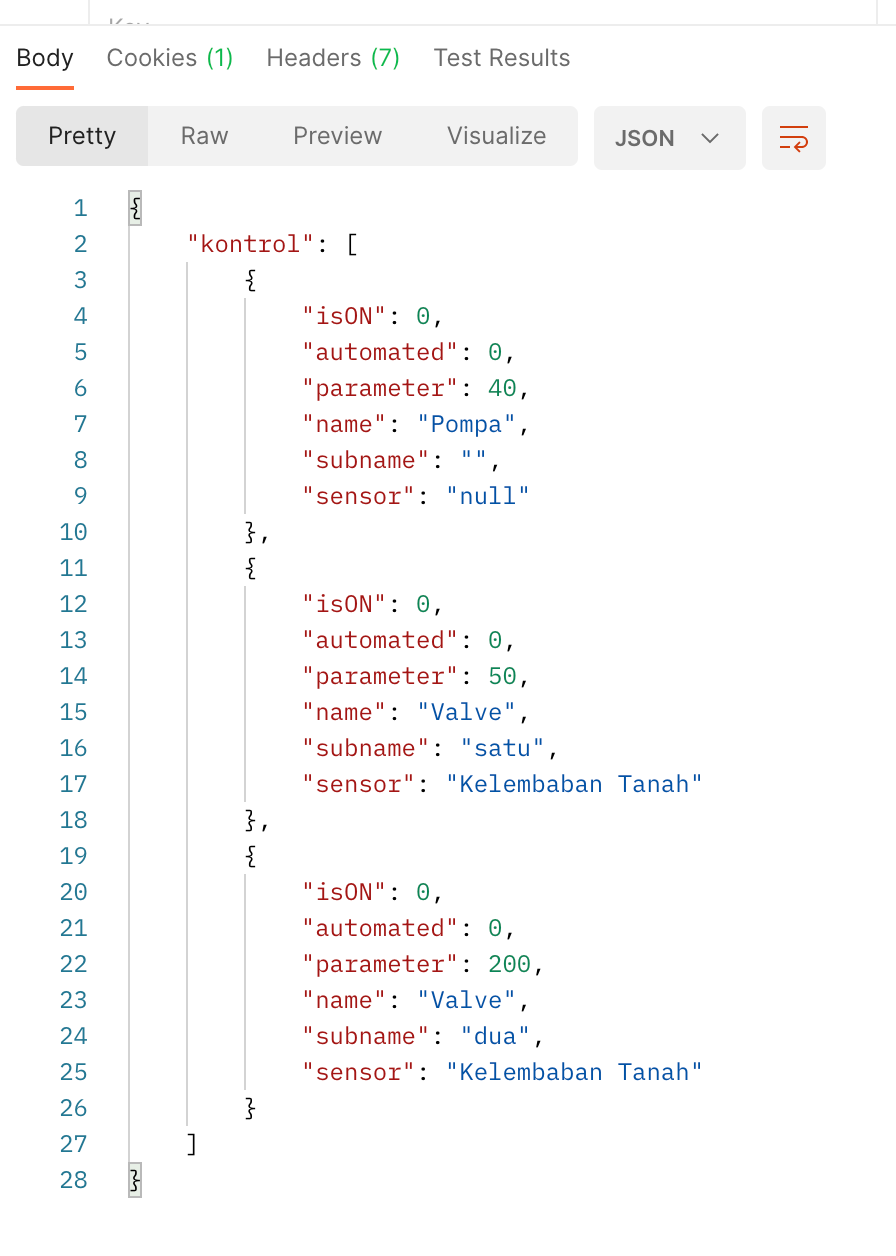
\includegraphics[width=11cm]{images/bab 4/api/kontrol.png}
                    \caption{API Data Kontrol}
                \end{figure}
                \item API data ikon\\
                http://47.89.212.89/dummyBackend/(\emph{endpoint}) \\
                (\emph{endpoint} berada pada API data \emph{realtime}) yang tertera pada Gambar 4.10\\
                Merupakan data yang menyimpan lokasi \emph{asset} ikon sensor.
                \item API status alat\\
                http://47.89.212.89/dummyBackend/status/(\emph{endpoint})\\
                Merupakan API yang berisikan data yang menunjukkan status keadaan alat.
                Berikut contoh tampilan API status alat
                dapat dilihat pada Gambar 4.12.
                \vspace{6cm}
                \begin{figure}[ht]
                    \centering
                    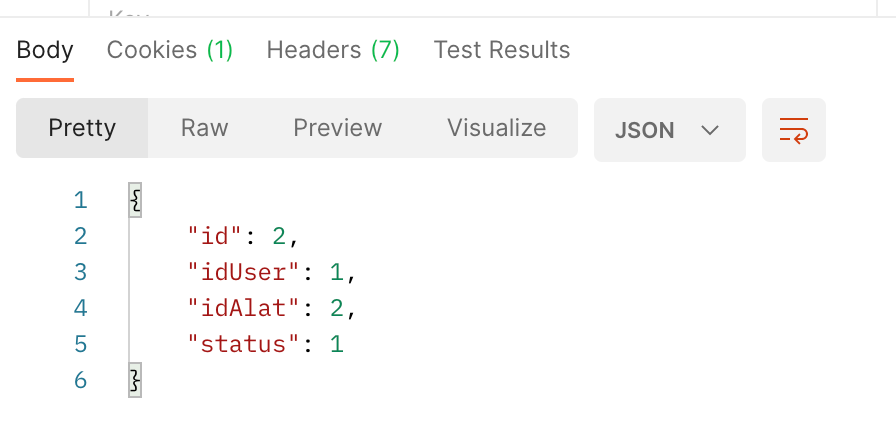
\includegraphics[width=11cm]{images/bab 4/api/status.png}
                    \caption{API Status Alat}
                \end{figure}
                \item API update kontrol\\
                http://47.89.212.89/dummyBackend/kontrol/(\emph{endpoint})\\
                Merupakan API untuk melakukan \emph{post} data update dari masukan pengguna.
            \end{itemize}
        API ini digunakan oleh peneliti dalam tahap pembuatan aplikasi \emph{mobile} KEBUNQ sebagai penghubung antara aplikasi dengan \emph{database server}.\\
        

        
% PEMODELAN PROSES
        \subsubsection{Pemodelan Proses}
        Berikut beberapa pemodelan proses aplikasi mobile KEBUNQ BPP Lampung yang dirancang setelah menganalisa tahap pemodelan bisnis dan 
            pemodelan data.
        \begin{enumerate}[label=\alph*.]
            \item \emph{Flowchart}\\
            \begin{figure}[ht]
                \centering
                \includegraphics[width=12cm]{images/bab 4/fc 1.png}
                \caption{\textit{flowchart} bagian 1 (mulai)}
            \end{figure}
            \vspace{12cm}
            \\\\Pada Gambar 4.13 menunjukkan proses  sejak dimulai hingga masuk ke halaman \emph{home}. Ketika dibuka, aplikasi akan menampilkan halaman \emph{splashscreen} kemudian melakukan pengecekan apakah pengguna sudah pernah
            melakukan login dengan benar atau belum, jika sudah pernah dan belum melakukan logout maka akan langsung masuk ke halaman \emph{home} dan jika belum, aplikasi akan menampilkan halaman \emph{login}. Pada halaman \emph{login} pengguna diharuskan memasukkan \emph{username} dan \emph{password} dengan benar untuk bisa masuk ke halaman \emph{home}.
            \vspace{8cm}
            \begin{figure}[ht]
                \centering
                \includegraphics[width=12cm]{images/bab 4/fc-kontrol.png}
                \caption{\textit{flowchart} bagian 2 (kontrol)}
            \end{figure}
            \\Pada Gambar 4.14 menunjukkan proses pengguna melakukan kontrol. Ketika pengguna memilih fitur kontrol langsung maka aplikasi akan mengirimkan data perintah \emph{on} atau \emph{off}
            ke server sehingga keadaan data menjadi sesuai dengan data aktual sebagaimana yang tampil pada aplikasi. 
            Jika tidak melakukan kontrol langsung, maka pengguna bisa melakukan perintah kontrol dengan mode otomatis., dalam proses tersebut pengguna diminta memberikan masukan berupa nilai parameter dan melakukan konfirmasi. Setelah itu data akan dikirim ke \emph{database} dan aplikasi akan menampilkan status kontrol tersebut berada pada mode otomatis.
            \begin{figure}[ht]
                \centering
                \includegraphics[width=8cm]{images/bab 4/fc-pilih alat.png}
                \caption{\textit{flowchart} bagian 3 (selesai)}
            \end{figure}
            \\Pada Gambar 4.15 menunjukkan proses yang terjadi ketika pengguna membuka menu yang terdapat beberapa opsi pilihan, yaitu (1) memilih alat yang akan ditampilkan datanya, (2) memilih untuk kembali ke halaman \emph{home}, dan (3) pengguna dapat melakukan \emph{logout}.
           
            \item \textit{Use Case}
            \begin{figure}[ht]
                \centering
                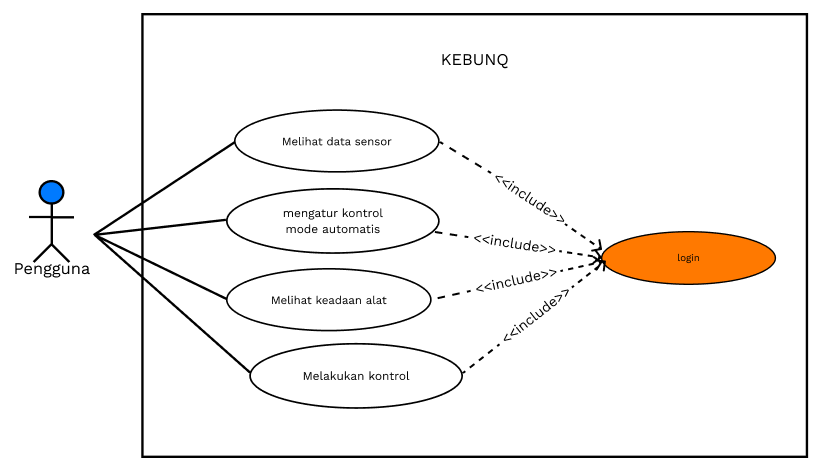
\includegraphics[width=10cm]{images/bab 4/use-case-user.png}
                \caption{\textit{Use Case Diagram}}
            \end{figure}
            \\Pada Gambar 4.16 menampilkan gambaran apa saja yang bisa dilakukan pengguna dalam aplikasi KEBUNQ, yaitu pengguna dapat melihat data sensor,
            melakukan kontrol secara langsung atau mode otomatis, dan melihat keadaan alat apakah \emph{offline / online}. Namun hal tersebut dapat dilakukan pengguna dengan syarat harus melakukan
            login terlebih dahulu.
            \item \textit{Sequence Diagram}
            \begin{figure}[ht]
                \centering
                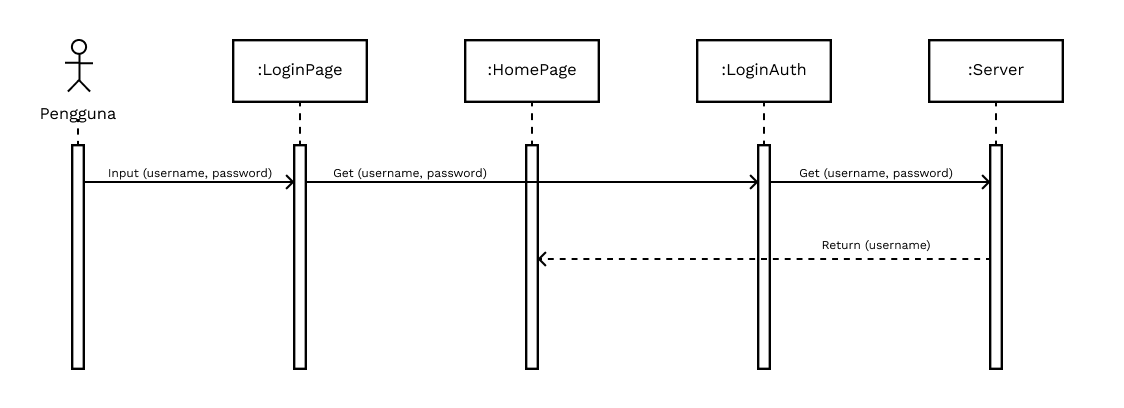
\includegraphics[width=12cm]{images/bab 4/Sequence login.png}
                \caption{\textit{Sequence Diagram Login}}
            \end{figure}
            \\Pada Gambar 4.17 menunjukkan gambaran proses ketika pengguna melakukan \emph{login}. Dimulai dengan pengguna memberikan \emph{input} \emph{username} dan \emph{password} pada halaman \emph{login}. Kemudian aplikasi melakukan \emph{authentication} atau proses pengecekan data apakah sesuai dengan yang tersedia pada server. Ketika data tersebut sesuai, maka aplikasi akan melakukan pengambilan data dan pada halaman \emph{home}
            akan menampilkan \emph{username} pengguna.\\
            \begin{figure}[ht]
                \centering
                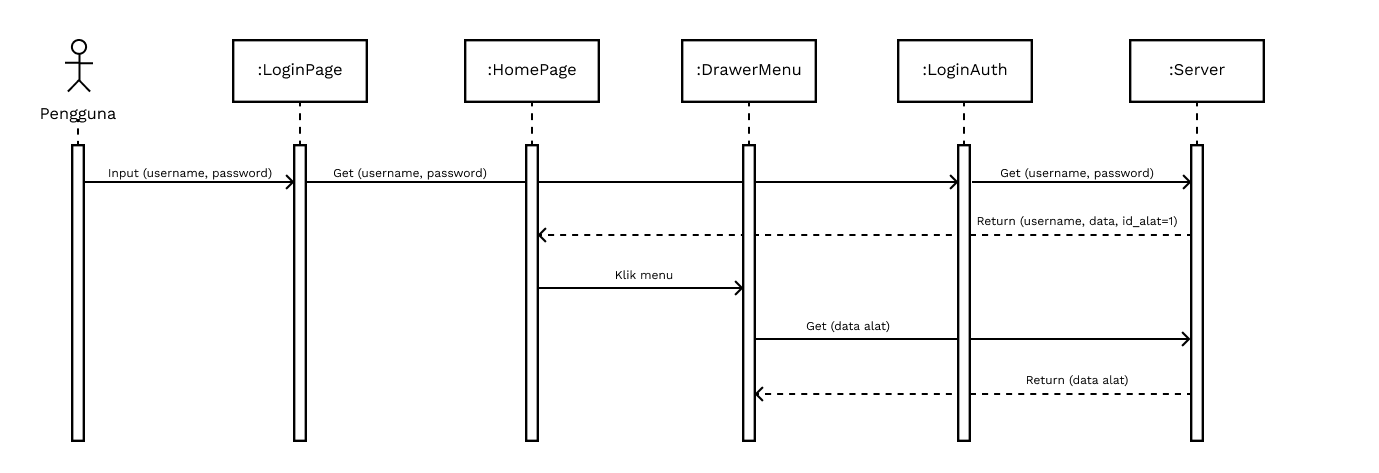
\includegraphics[width=12cm]{images/bab 4/buka menu alat.png}
                \caption{\textit{Sequence Diagram} Melihat Menu / Alat}
            \end{figure}
            \\Pada Gambar 4.18 menunjukkan gambaran proses ketika pengguna melihat menu. Setelah melewati proses \emph{login}, pengguna memilih menu pada halaman \emph{home} kemudian aplikasi akan melakukan pengambilan data ke server dan menampilkan hasilnya pada menu.
            \begin{figure}[ht]
                \centering
                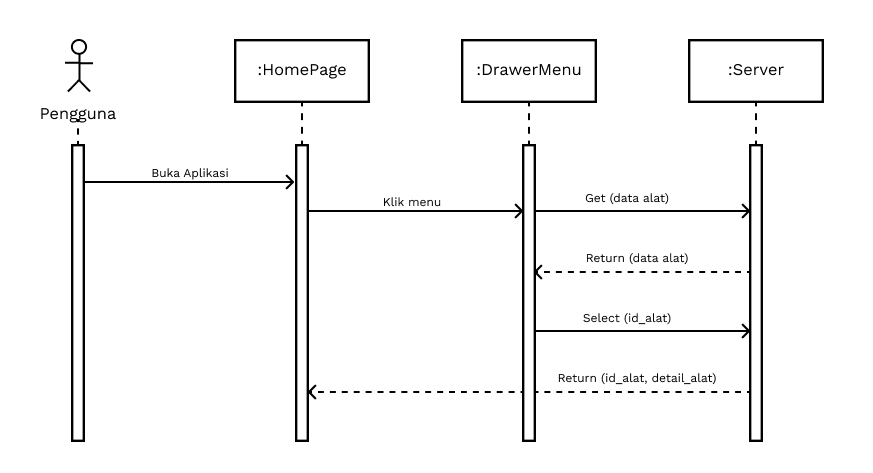
\includegraphics[width=10cm]{images/bab 4/Sequence buka detail alat.png}
                \caption{\textit{Sequence Diagram} Melihat Detail Alat}
            \end{figure}
            \\Pada Gambar 4.19 menunjukkan gambaran proses ketika pengguna melihat data yang ada pada suatu alat. Dimulai dengan pengguna membuka aplikasi dan setelah berada pada halaman \emph{home} pengguna memilih menu sehingga tampil bagian \emph{drawer}/menu alat yang ada, setelah itu pengguna dapat memilih alat yang berada pada menu tersebut dan aplikasi akan melakukan pengiriman data id yang dipilih ke server, 
            kemudian aplikasi akan menampilkan data yang ada dari alat tersebut pada halaman \emph{home}.
            \vspace{4cm}
            \begin{figure}[ht]
                \centering
                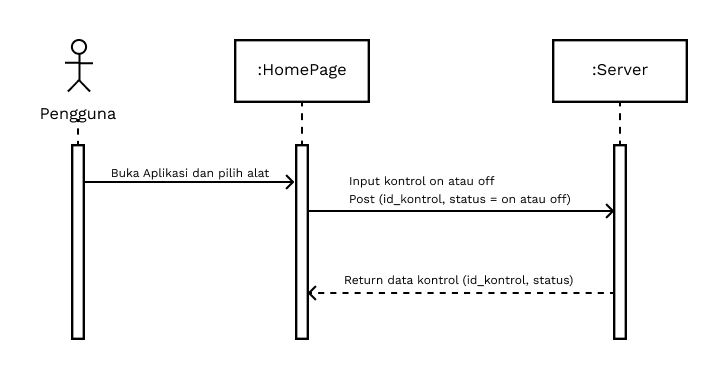
\includegraphics[width=12cm]{images/bab 4/Sequence kontrol.png}
                \caption{\textit{Sequence Diagram} Melakukan Kontrol}
            \end{figure}
            \\Pada Gambar 4.20 menunjukkan gambaran proses ketika pengguna melakukan kontrol. Setelah berada pada halaman \emph{home} dan menampilkan bagian alat yang terpilih, pengguna dapat menginputkan kontrol \emph{on/off} kemudian aplikasi akan menampilkan data sesuai dengan yang tersedia pada server.
            \begin{figure}[ht]
                \centering
                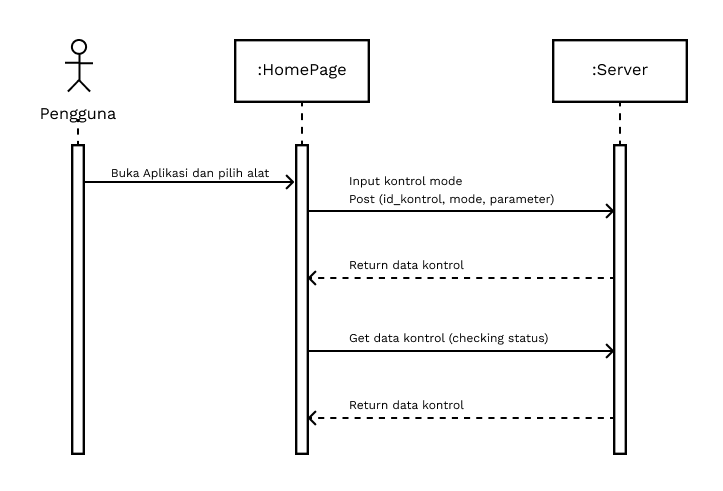
\includegraphics[width=11cm]{images/bab 4/Sequence kontrol Auto.png}
                \caption{\textit{Sequence Diagram} Melakukan Kontrol Automatis}
            \end{figure}
            \\Pada Gambar 4.21 menunjukkan gambaran proses ketika pengguna melakukan kontrol otomatis. Dimulai dengan keadaan pengguna yang sudah berada pada tampilan alat yang akan dikontrol memilih kontrol mode otomatis dan memasukkan nilai parameter kontrol tersebut, kemudian aplikasi akan menampilkan data aktual sebagaimana data yang berada pada server.
            \end{enumerate}

        \subsubsection{Pembuatan Aplikasi}
        Dalam proses pembuatan aplikasi peneliti melakukan 3 pengerjaan (1) Perancangan desain layout \textit{User Interface}, (2) Pembuatan \textit{assets} mencakup logo aplikasi, ikon sensor, dan ilustrasi kontrol, dan (3) Pengerjaan pembuatan aplikasi menggunakan \textit{framework} Flutter dengan bahasa pemrograman Dart
        \begin{enumerate}
            \item Perancangan Desain Layout \textit{User Interface}
            \begin{figure}[ht]
                \centering
                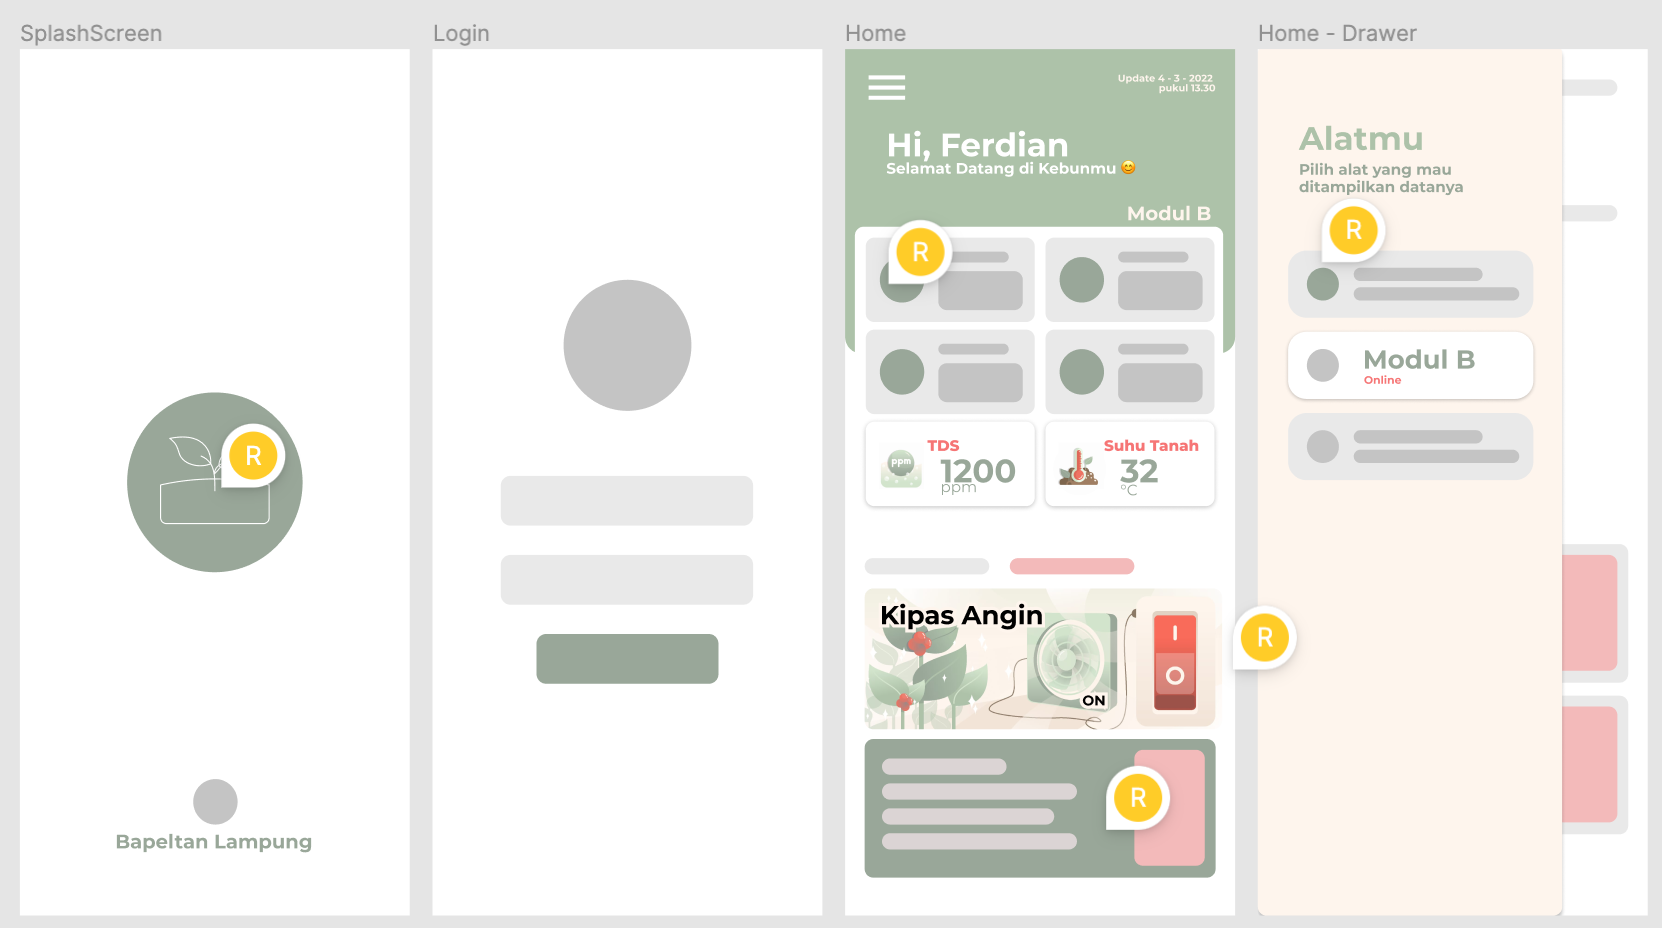
\includegraphics[width=13cm]{images/UI/summary.png}
                \caption{Rancangan layout UI}
            \end{figure}
            \\Pada Gambar 4.22 terdapat beberapa halaman yang dibuat berupa \emph{layout} untuk memudahkan pembuatan aplikasi. Halaman
            tersebut yaitu halaman \emph{splashscreen}, halaman \emph{login}, halaman \emph{home} dan tampilan menu \emph{drawer}.\\
            \item Pembuatan \textit{assets}\\
            \begin{figure}[ht]
                \centering
                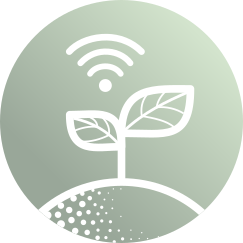
\includegraphics[width=5cm]{images/logo.png}
                \caption{\textit{assets} Logo aplikasi}
            \end{figure}
            \noindent \\Logo aplikasi KEBUNQ pada Gambar 4.23 dirancang memiliki arti sebagai berikut :
            \begin{itemize}
                \item Bentuk koin : menunjukkan bahwa aplikasi KEBUNQ dirancang untuk mendukung program \emph{low cost smart farming}
                \item Tanda sinyal : menunjukkan penggunaan aplikasi memerlukan konektivitas jaringan internet untuk melakukan pemantauan dan kontrol dari jarak jauh (\emph{online apps})
                \item Tanaman : menunjukkan bahwa aplikasi KEBUNQ berhubungan erat dan tidak lepas dengan tanaman dalam penggunaannya
                \item pijakan tanaman dan bulatan-bulatan kecil : mewakilkan banyaknya unsur yang dapat kita pantau melalui aplikasi KEBUNQ.\\\\
            \end{itemize}
            \begin{figure}[ht]
                \centering
                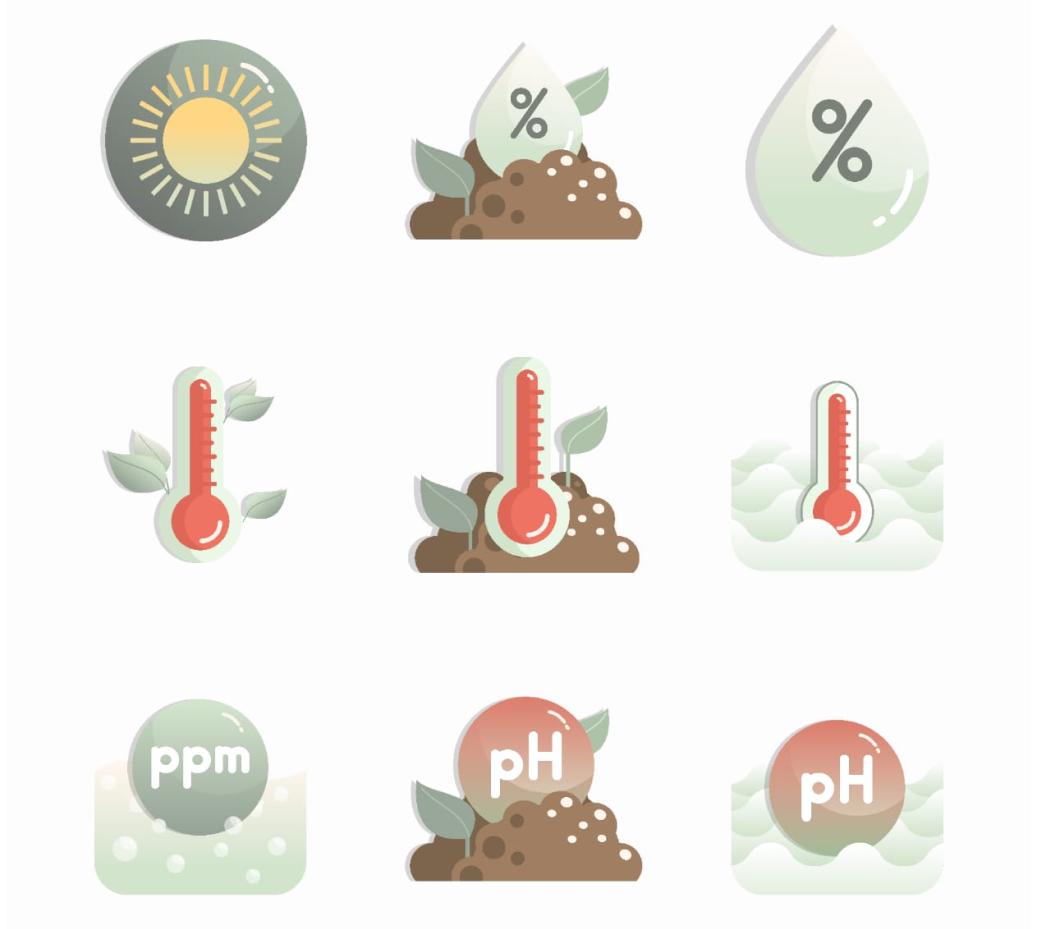
\includegraphics[width=10cm]{images/UI/ikon.png}
                \caption{\textit{assets} Ikon Sensor}
            \end{figure}
            \noindent Pada Gambar 4.24 tercantum \emph{asset} ikon sensor yang akan digunakan untuk ditampilkan pada aplikasi. Terdapat 9 buah ikon sebagaimana yang tercantum dalam hasil observasi.
            \begin{figure}[ht]
                \centering
                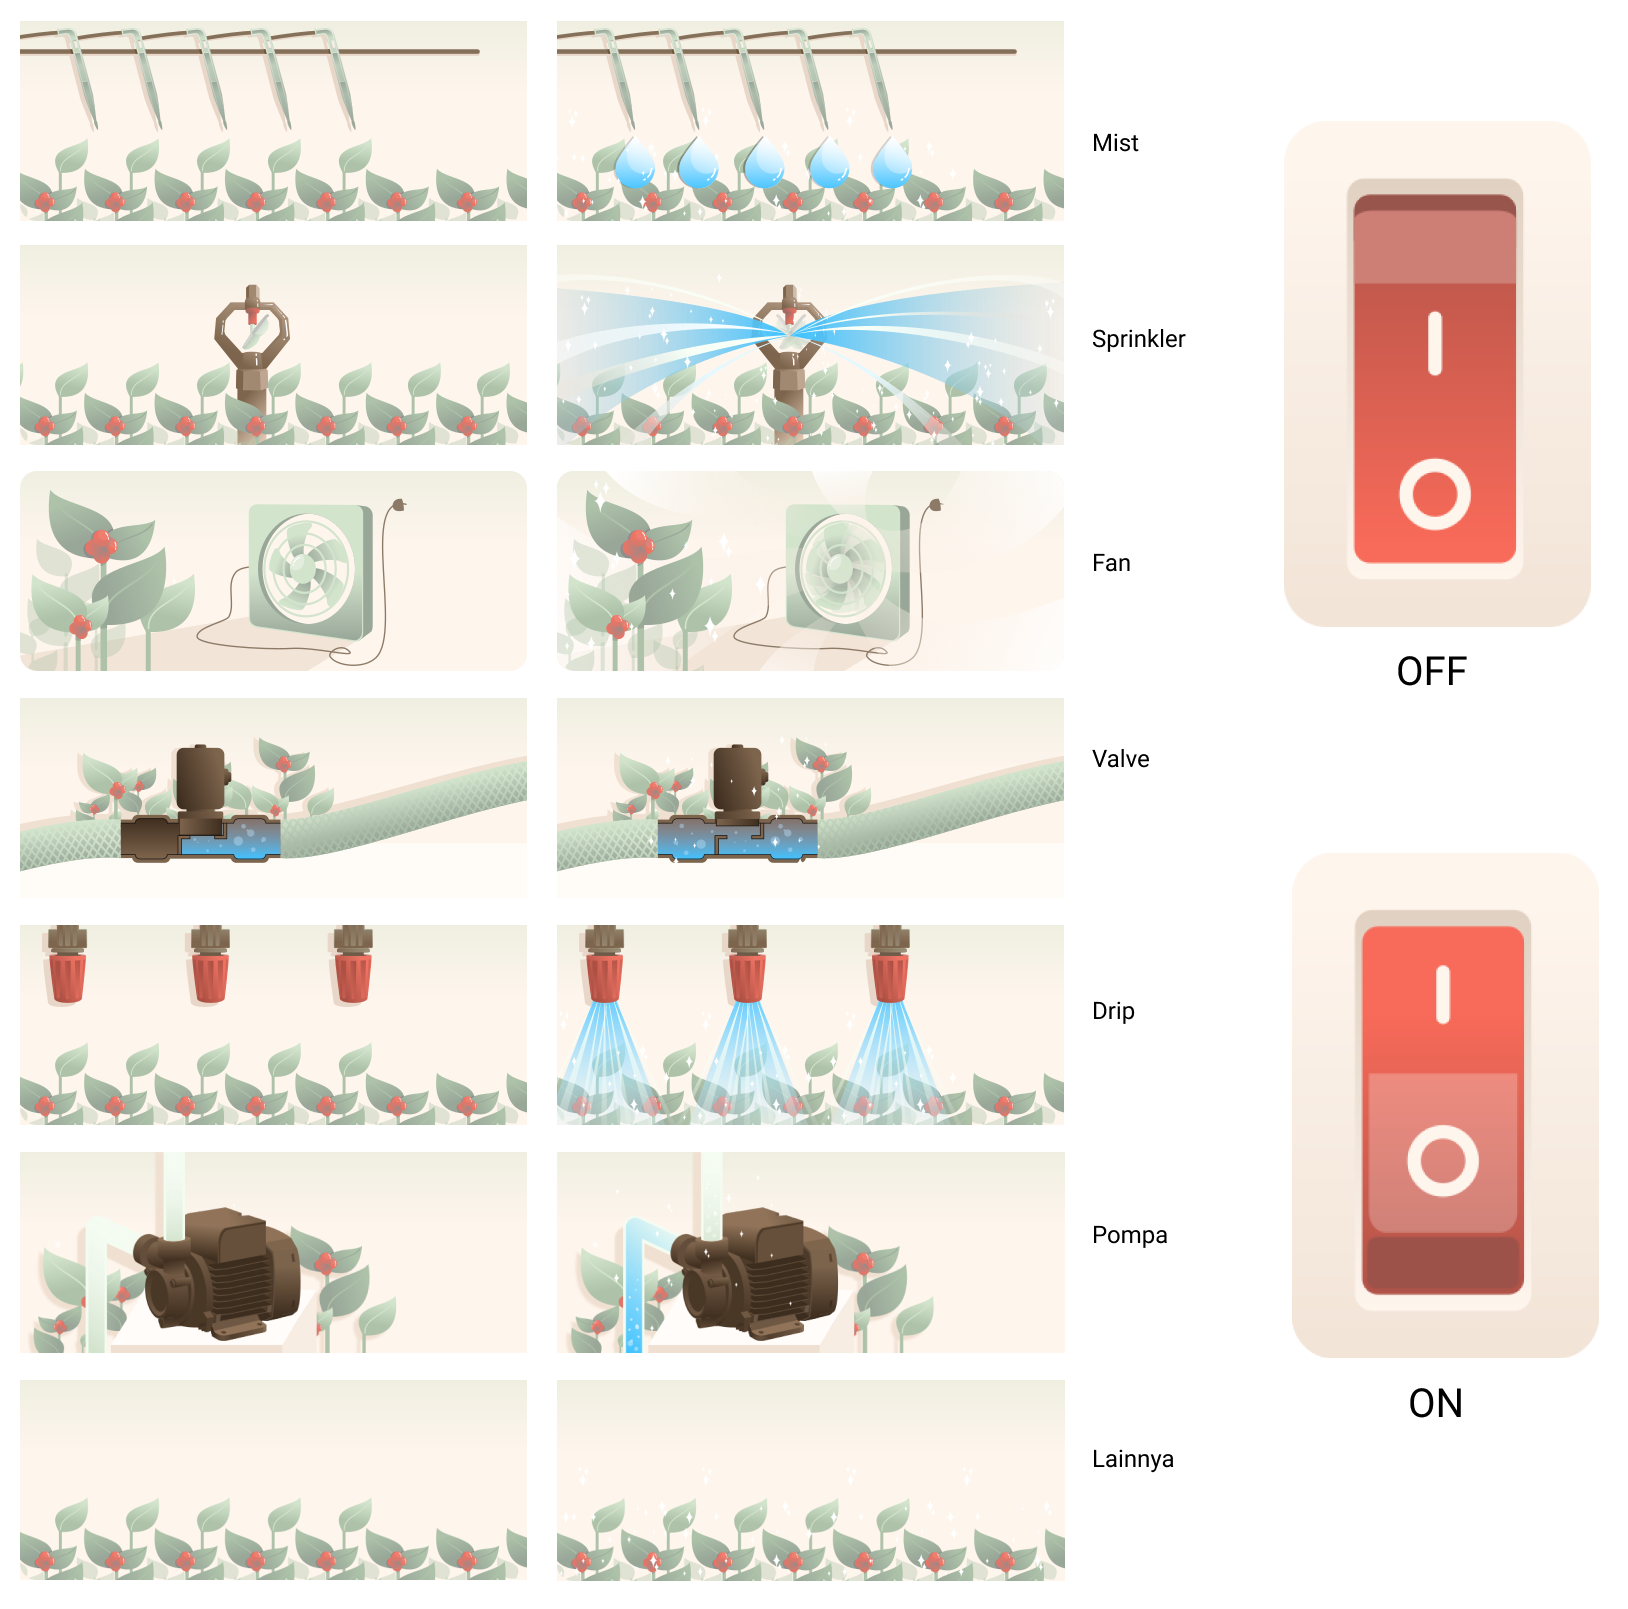
\includegraphics[width=12cm]{images/UI/Frame 1.png}
                \caption{\textit{assets} Kontrol}
            \end{figure}
            \vspace{3cm}
            \noindent \\Pada Gambar 4.25 mencantumkan \emph{assets} yang akan digunakan pada tampilan kontrol alat, desain yang dibuat tersebut berdasarkan data hasil observasi. Pembuatan \emph{assets} logo, ikon dan ilustrasi bertujuan untuk meningkatkan kemudahan pengguna dalam menggunakan aplikasi KEBUNQ dan menjadikan KEBUNQ sebagai aplikasi yang unik dengan menggunakan \emph{assets} yang orisinil khusus didesain dan digunakan pada aplikasi KEBUNQ. \\
            \item Pembuatan Aplikasi\\
            Implementasi dari perancangan aplikasi KEBUNQ
            \begin{itemize}
                \item Halaman \emph{Splash Screen}\\
                Merupakan halaman pertama yang dilihat dengan hitungan waktu beberapa detik. Pada aplikasi KEBUNQ, \emph{splash screen} dibuat dengan sedikit implementasi gerak animasi dan mencantumkan logo KEBUNQ dan BPP Lampung.
                Halaman \emph{Splash Screen} dapat dilihat pada Gambar 4.26.
                \begin{figure}[ht]
                    \centering
                    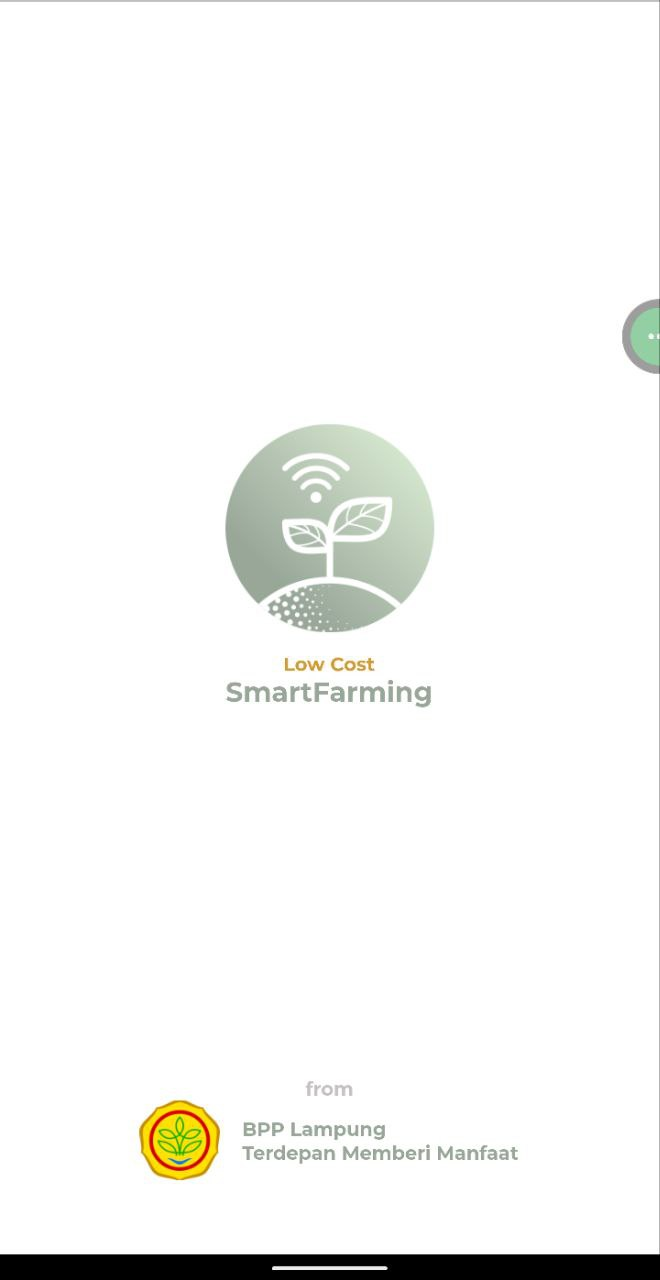
\includegraphics[width=8cm]{images/bab 4/splash.jpeg}
                    \caption{Tampilan \emph{Splash Screen}}
                \end{figure}
                \item Halaman \emph{Login}\\
                Halaman \emph{login} berupa formulir \emph{login} yang diharuskan untuk diisi dengan benar supaya kemudian pengguna dapat menggunakan fitur utama aplikasi KEBUNQ. Halaman login menampilkan \emph{field username} dan \emph{password}.
                Dalam proses \emph{login} dilakukan pemeriksaan data apakah data yang dimasukkan sesuai dengan \emph{database} atau tidak. Jika ada maka aplikasi KEBUNQ akan menampilkan halaman \emph{Home} dan menampilkan data yang dimiliki oleh pengguna. \
                Halaman \emph{login} dapat dilihat pada Gambar 4.27.
                \begin{figure}[ht]
                    \centering
                    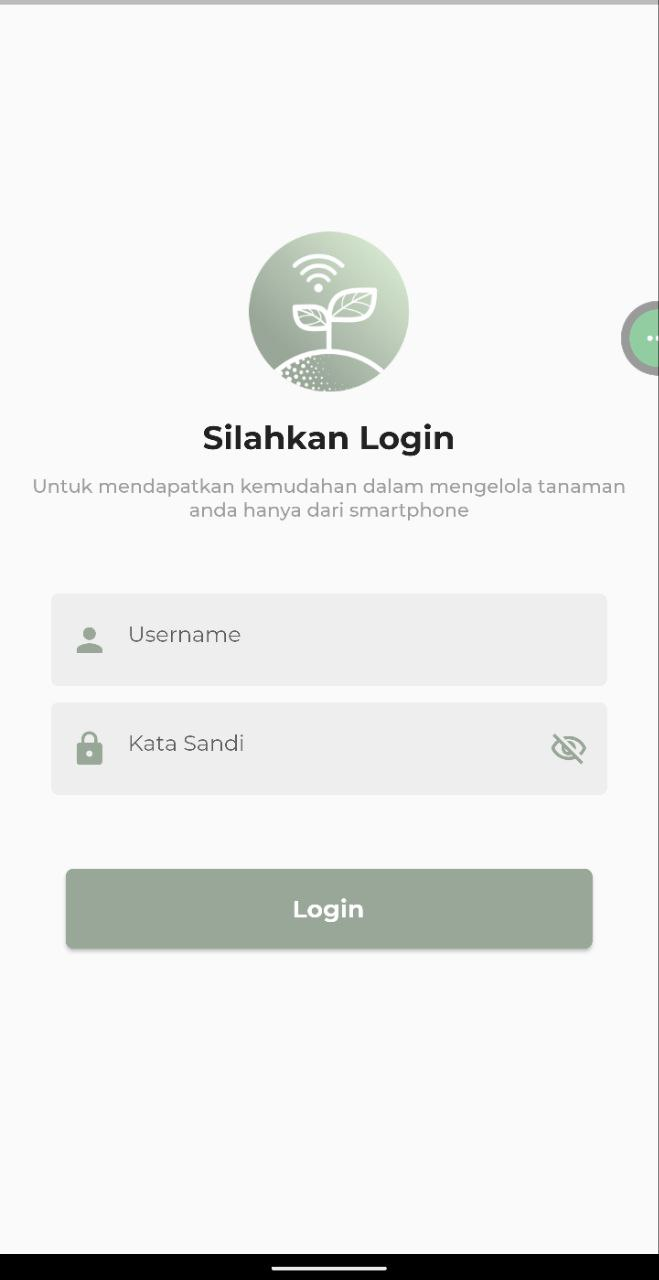
\includegraphics[width=8cm]{images/bab 4/login.jpeg}
                    \caption{Tampilan Halaman \emph{Login}}
                \end{figure}
                \vspace{10cm}
                \item Halaman \emph{Home}\\
                Halaman \emph{Home} merupakan halaman utama yang digunakan pengguna untuk melihat data sensor dan kontrol yang ada. Pengguna dapat melakukan kontrol atau kendali dengan cara menyalakan atau mematikan kontrol maupun memberikan \emph{setting} automatis pada kontrol yang dipilih.
                Halaman \emph{Home} dapat dilihat pada Gambar 4.28.
                \begin{figure}[ht]
                    \centering
                    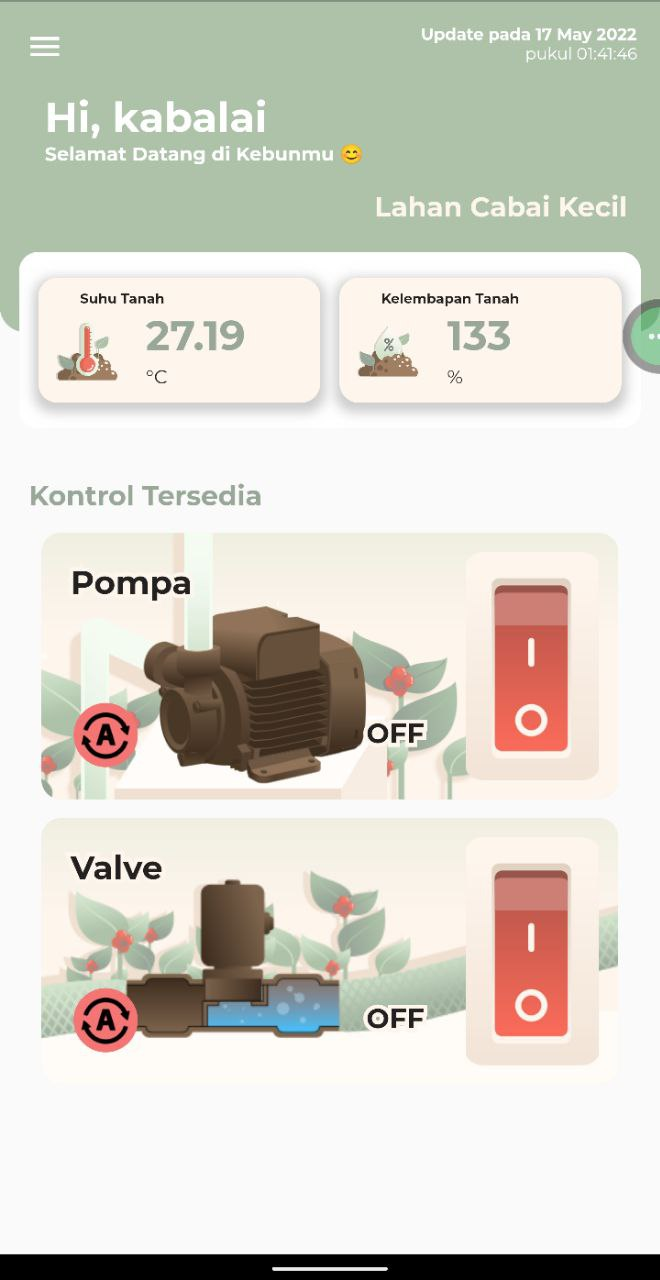
\includegraphics[width=8cm]{images/bab 4/home.jpeg}
                    \caption{Tampilan Halaman \emph{Home}}
                \end{figure}
                \newline
                \vspace{10cm}
                \item \emph{Drawer}\\
                \emph{Drawer} merupakan bagian tampilan Menu yang terdapat pada halaman \emph{Home} ketika diklik/disentuh. Menu \emph{drawer} berisikan \emph{list} alat yang tersedia pada akun pengguna. Pada \emph{list} alat tersebut terdapat nama alat dan status keadaan alat sekarang apakah \emph{online} (keadaan nyala) atau \emph{offline} (keadaan mati).
                Tampilan menu \emph{drawer} dapat dilihat pada Gambar 4.29.
                \begin{figure}[ht]
                    \centering
                    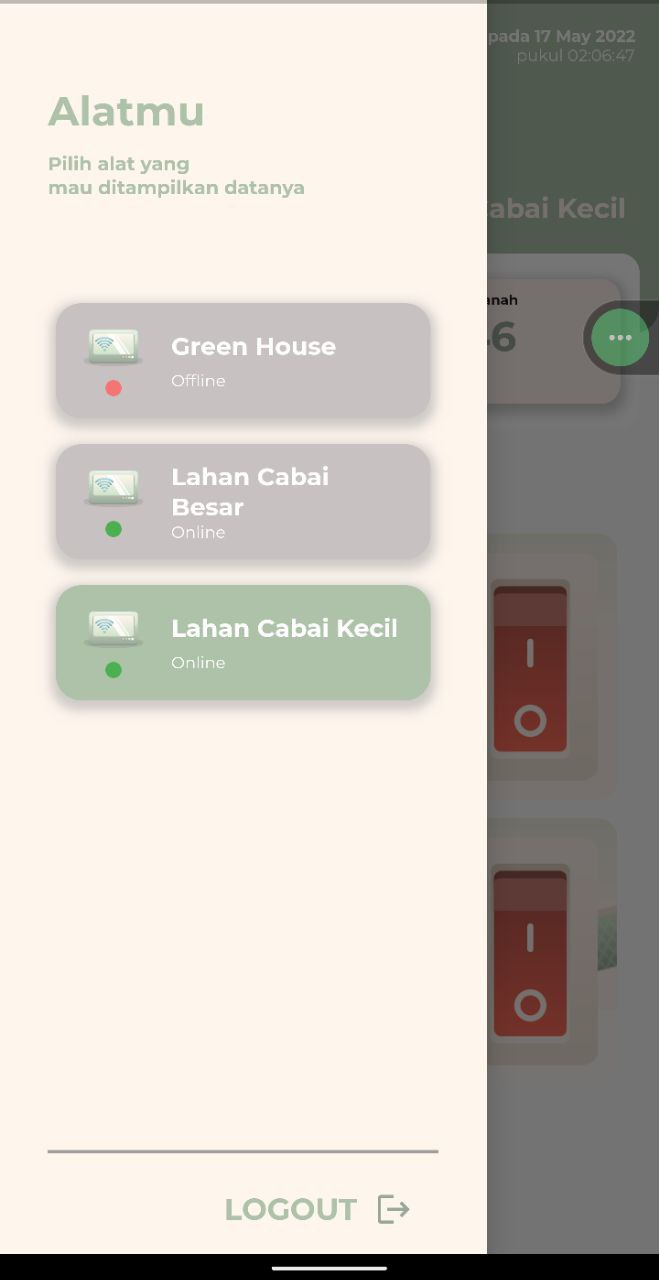
\includegraphics[width=8cm]{images/bab 4/drawerr.jpeg}
                    \caption{Tampilan Menu \emph{Drawer}}
                \end{figure}
                \vspace{10cm}
                \item Tampilan \emph{Loading}
                Tampilan \emph{loading} merupakan tampilan yang muncul membentuk \emph{shimmer} pada layout yang dibuat ketika aplikasi KEBUNQ menunggu \emph{loading request} data dari API.
                Tampilan \emph{loading} dapat dilihat pada Gambar 4.30.
                \vspace{10cm}
                \begin{figure}[ht]
                    \centering
                    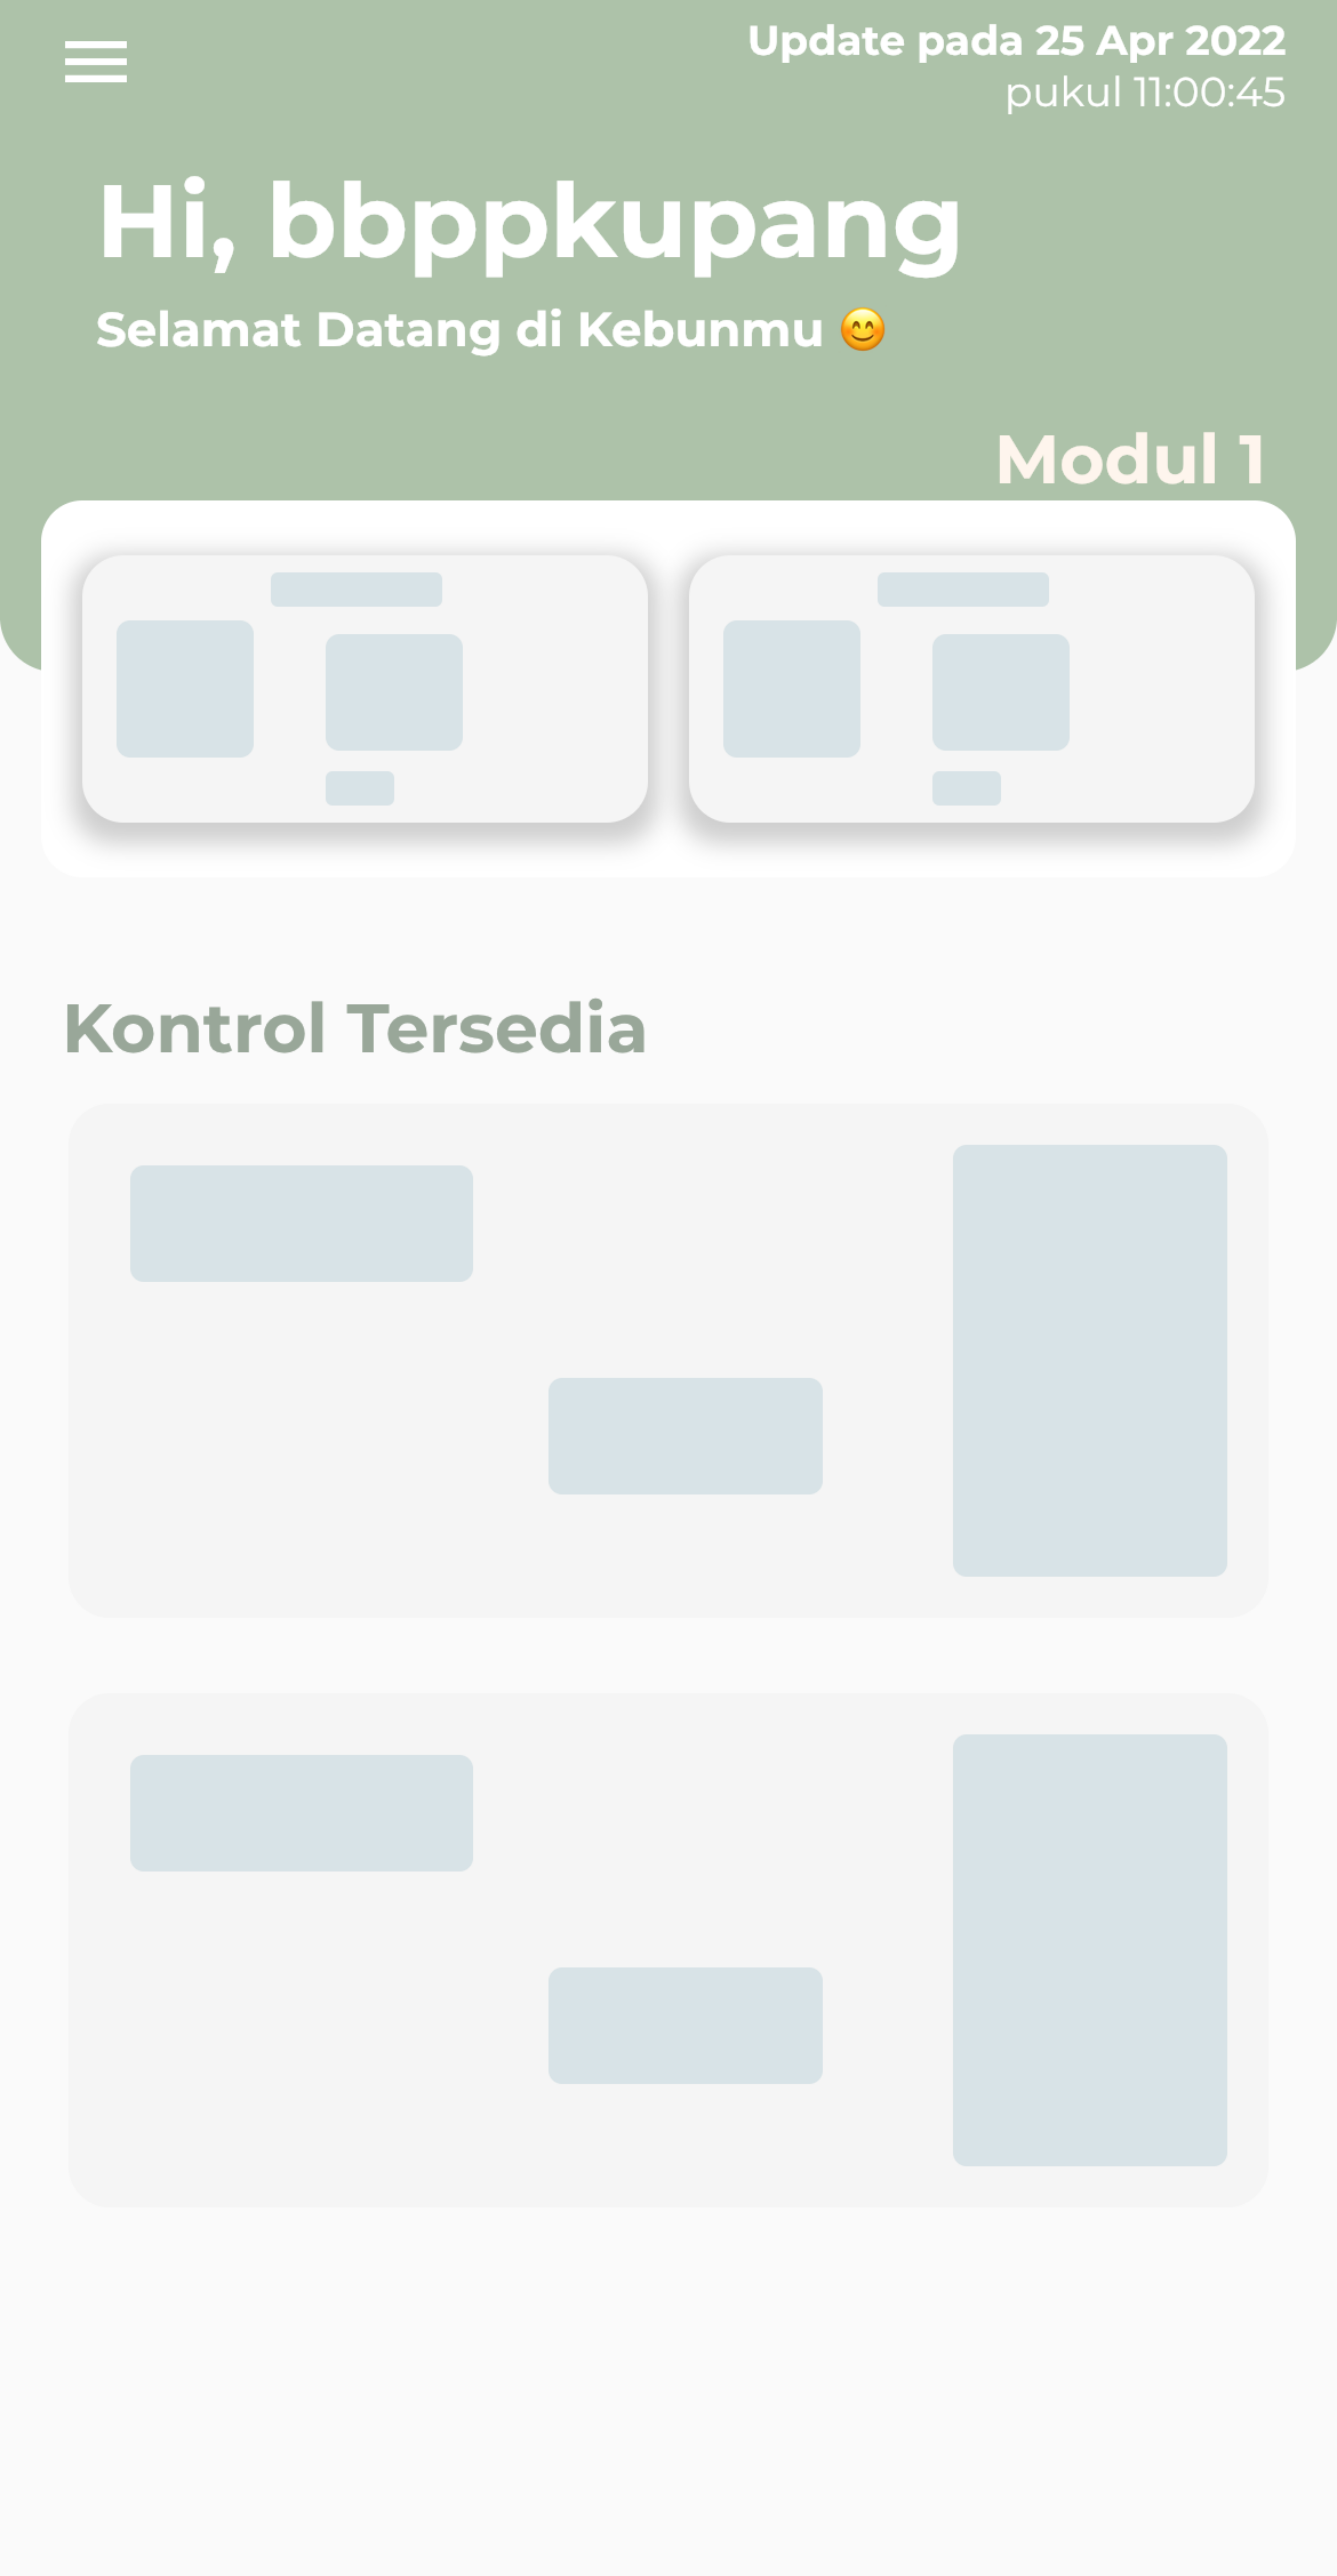
\includegraphics[width=8cm]{images/bab 4/ui-loading.png}
                    \caption{Tampilan \emph{Loading}}
                \end{figure}

            \end{itemize}
        \end{enumerate}
        Bersamaan dengan proses pembuatan aplikasi, sebagaimana tertera pada Gambar 4.7 Halaman 20 
        dilakukan juga pengerjaan perancangan alat yang dikerjakan oleh anggota tim. Alat yang dibuat tersebut merupakan alat
        yang akan dipasang pada lahan cabai besar, lahan cabai kecil, dan \emph{screen} hidroponik. 
        Pada lahan cabai besar alatnya menggunakan Esp32, \emph{soil capasitive sensor}, \emph{one wire temperature sensor}, dan modul relay 4 \emph{channel}.
        Pada lahan cabai kecil alatnya menggunakan Esp32, \emph{soil capasitive sensor}, \emph{one wire temperature sensor}, dan modul relay 2 \emph{channel}.
        Pada lahan \emph{screen} hidroponik alatnya menggunakan Esp32, DHT21, lux sensor BH1750, dan modul relay 2 \emph{channel}. 
        Berikut hubungan rancangan alat secara umum dapat dilihat pada Gambar 4.31.
        \begin{figure}[ht]
            \centering
            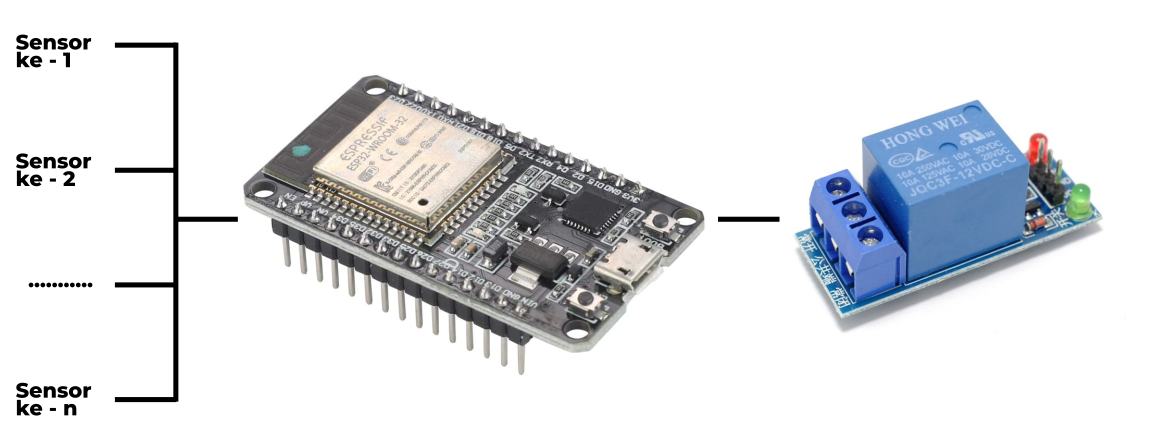
\includegraphics[width=12cm]{images/bab 4/alats.png}
            \caption{Rancangan Alat Secara Umum}
        \end{figure}
        \\Pada Gambar 4.31 dapat kita lihat ada 3 komponen utama dari alat yang dirancang yaitu 
        \emph{microcontroller} Esp32, sensor dan relay yang jumlahnya menyesuaikan dengan kebutuhan. 
        Aplikasi sudah dirancang akan otomatis mendukung jumlah sensor dan kontrol yang dinamis sesuai dengan 
        \emph{database}. Untuk detail rancangan alat, berikut salah satu rancangan skematik dari alat yang 
        dibuat untuk penggunaan pada lahan cabai dapat dilihat pada Gambar 4.32.
        \begin{figure}[ht]
            \centering
            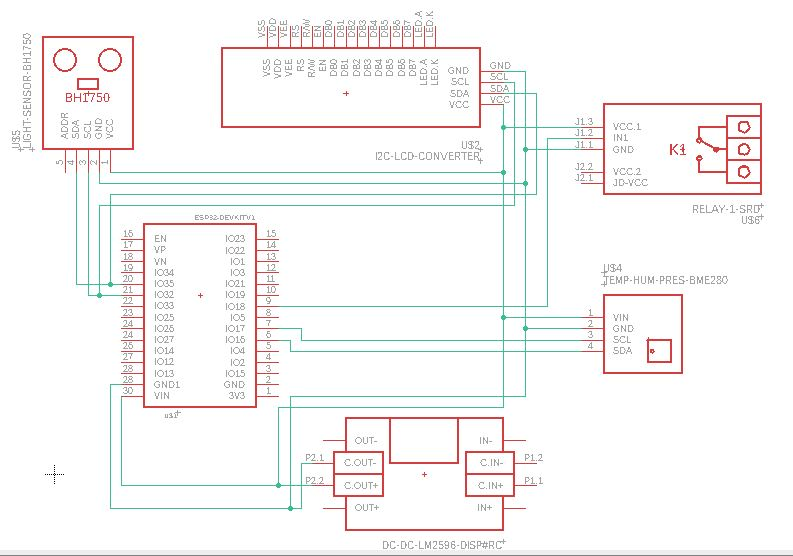
\includegraphics[width=12cm]{images/bab 4/Modul Ruangan.JPG}
            \caption{Rancangan Skematik Alat Lahan Cabai}
        \end{figure}
        \\Pada Gambar 4.32 menunjukkan skematik dari alat yang dibuat untuk lahan cabai yang menggambarkan hubungan
        dan alur antar pin dari komponen yang ada.
        \vspace{8cm}
        \begin{figure}[ht]
            \centering
            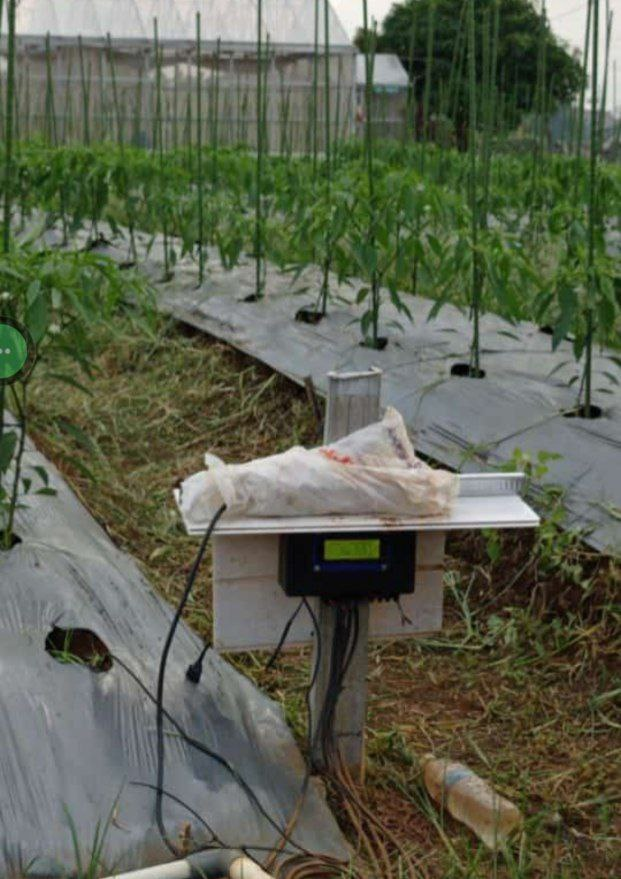
\includegraphics[width=10cm]{images/bab 4/gunain.jpeg}
            \caption{Alat Terpasang di Lahan}
        \end{figure}
        \\Pada Gambar 4.33 menunjukkan alat yang terpasang dan digunakan pada lahan cabai di BPP Lampung.\\

            \subsubsection{Pengujian dan Pergantian}
            Pada \emph{testing} aplikasinya menggunakan \emph{black box testing} untuk mencari tahu apakah aplikasi 
            sudah seperti yang dirapkan atau belum. Berikut beberapa tes yang dilakukan dapat dilihat pada Tabel 4.1 dan Tabel 4.2
            \begin{itemize}
                \item Pengujian Halaman \emph{Login}
                \vspace{6cm}
                \begin{table}[ht]
                    \centering
                    \caption{Pengujian Halaman \emph{Login}}
                    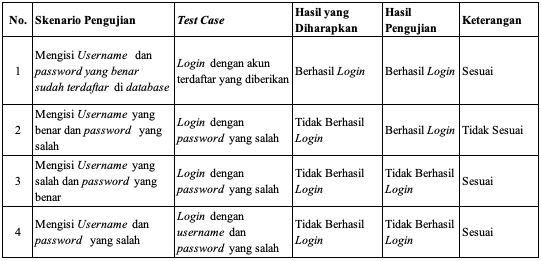
\includegraphics[width=12cm]{images/bab 4/fungsional-login.png}\\
                    \end{table}
                    \\Pada Tabel 4.1 dapat dilihat dari  \emph{test case} yang dilakukan untuk melihat apakah fungsionalitas pada halaman \emph{login} sudah sesuai atau belum dengan hasil yang diharapkan. Hasilnya adalah semua \emph{test case} sesuai dengan yang diharapkan setelah beberapa kali perbaikan ketika ditemukan bagian yang tidak sesuai.
                \item Pengujian Halaman \emph{Home}\\
                \begin{table}[ht]
                    \centering
                    \caption{Pengujian Halaman \emph{Home}}
                    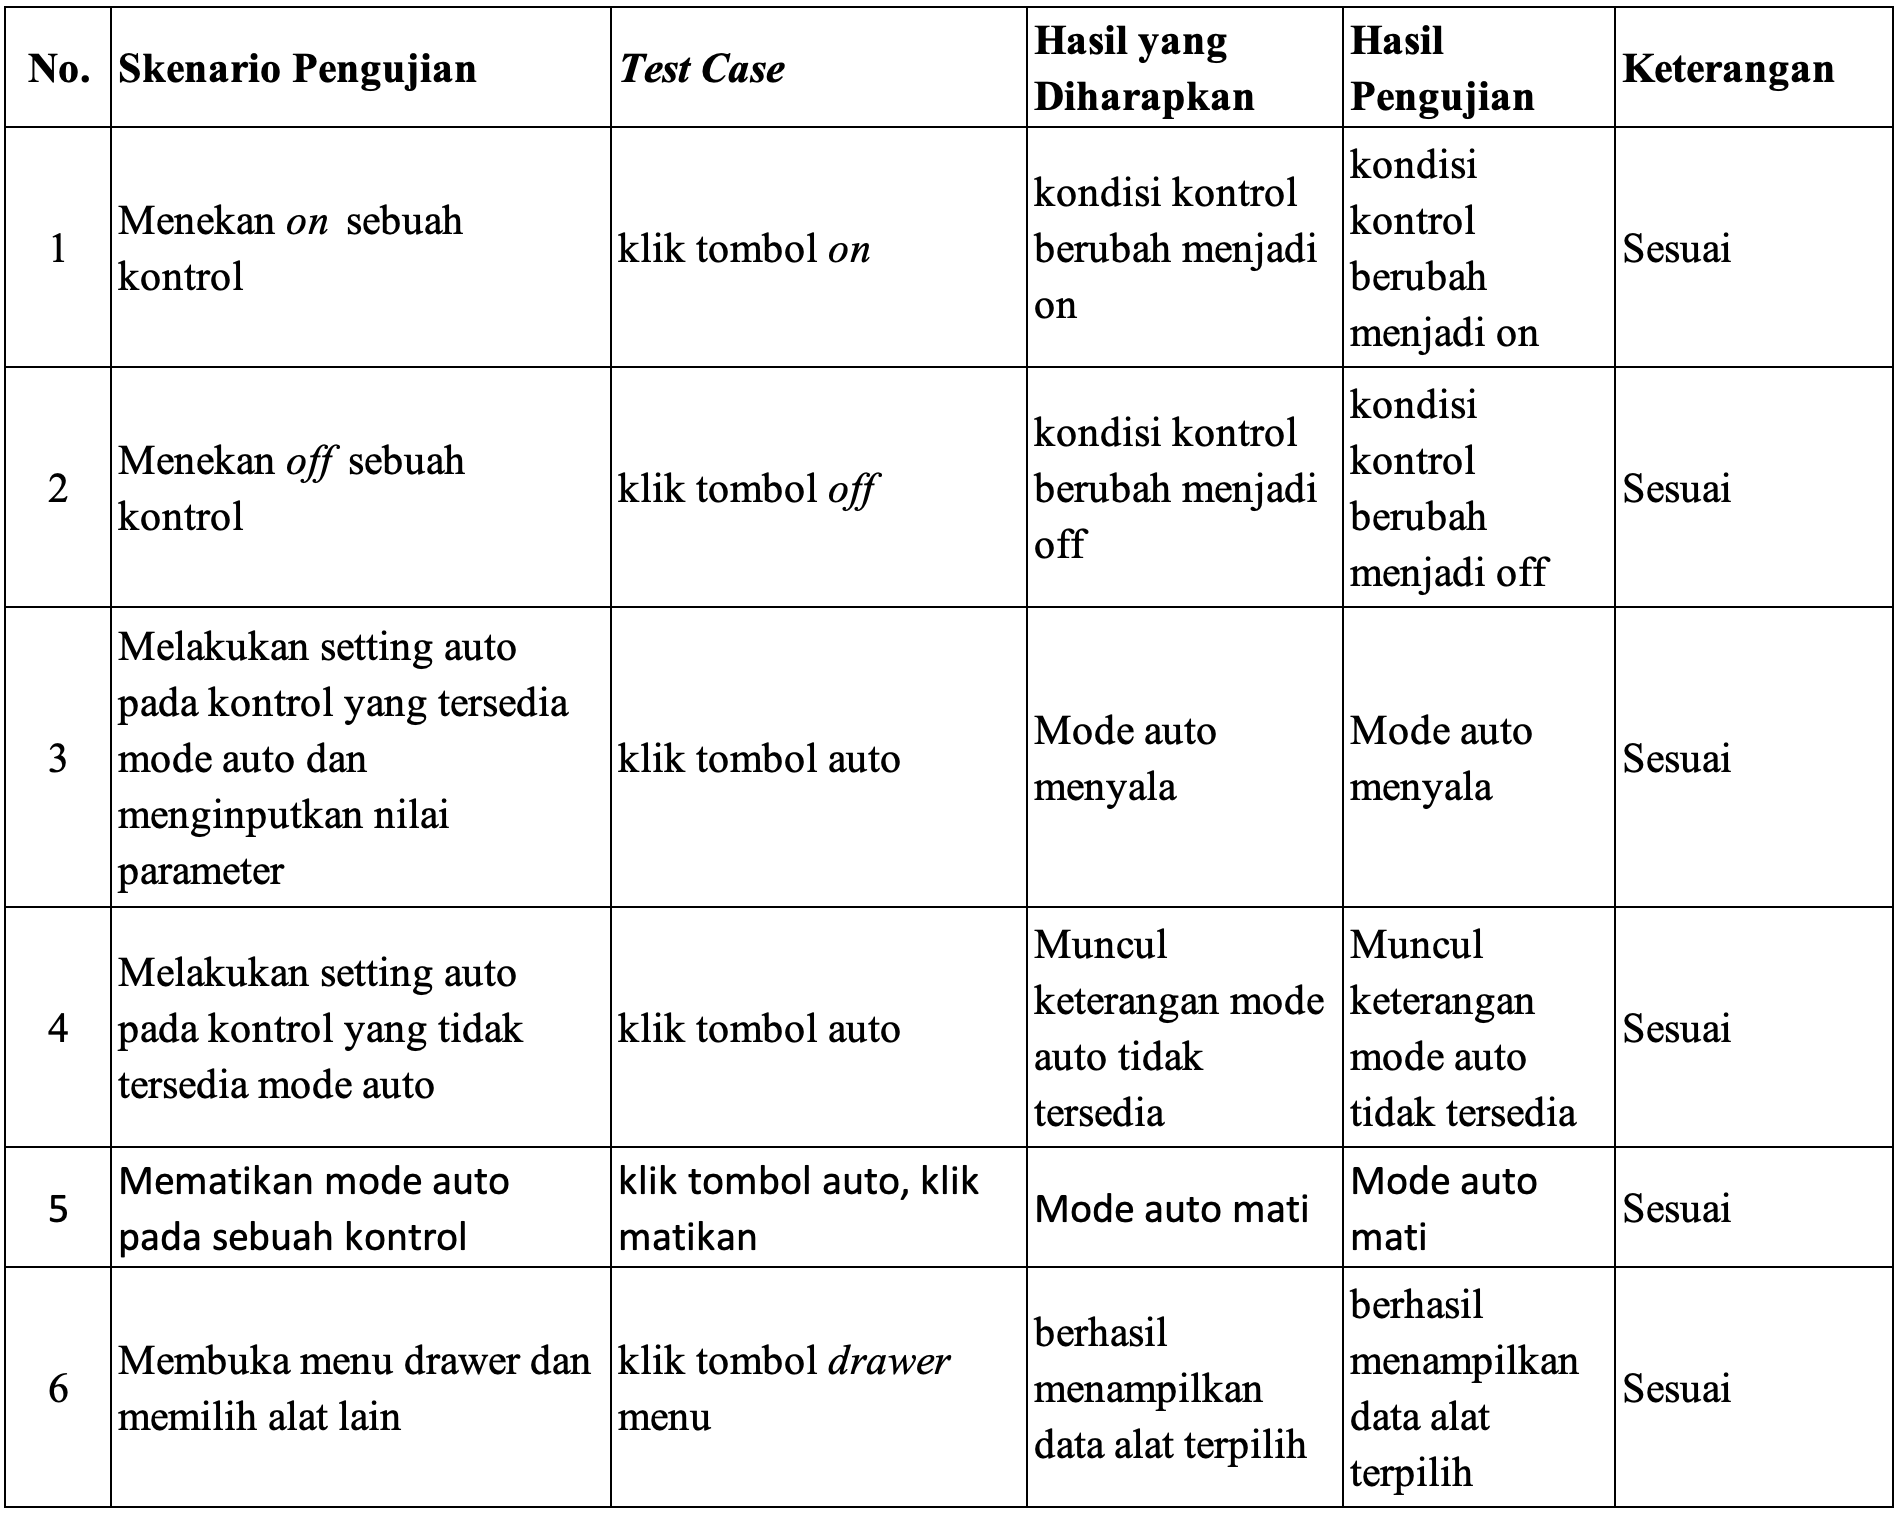
\includegraphics[width=12.5cm]{images/bab 4/fungsional-home1.png}\\
                    \end{table}
                \begin{table}[ht]
                    \centering
                    % \caption{Pengujian Halaman \emph{Home}}
                    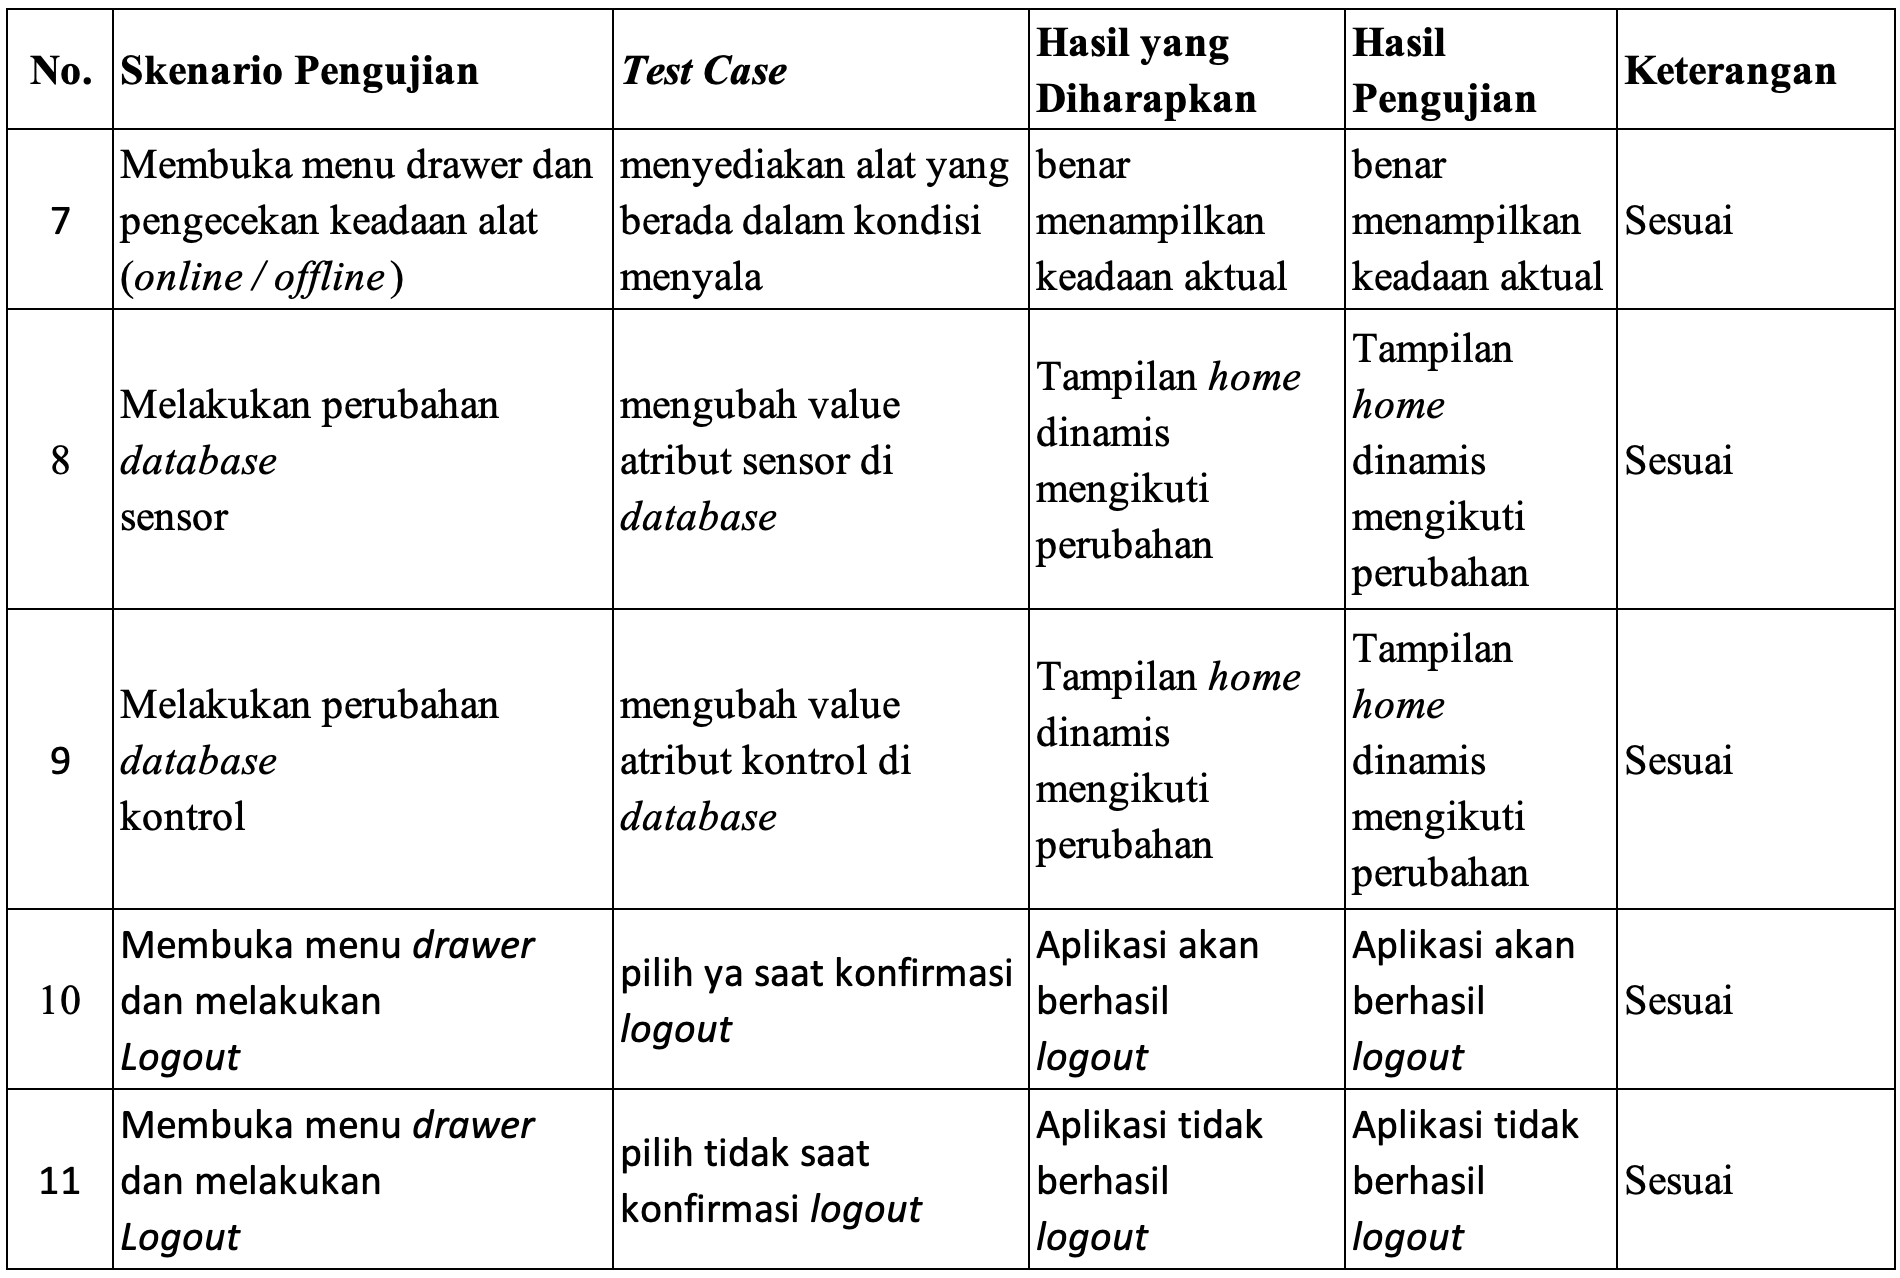
\includegraphics[width=13cm]{images/bab 4/fungsional-home2.png}\\
                    \end{table}
                \\[2cm]Pada Tabel 4.2 tertera fungsionalitas pada halaman \emph{home} dari 11 \emph{test case} yang disediakan, hasil akhirnya menunjukkan semua seuai dengan yang diharapkan.\\
            \end{itemize}
           
% \begin{table}[ht]
% \centering
% \caption{Permasalahan dan Solusinya}
% \begin{tabular}{|>{\raggedright}p{5cm}|p{2.5cm}|>{\raggedright}p{5cm}|}
%  \hline
%  \multicolumn{1}{|c}{\bfseries Masalah} & \multicolumn{1}{|c|}{\bfseries Aktor} & \multicolumn{1}{c|}{\bfseries Solusi} \\ 
%   \hline
% \begin{enumerate}
%    	\item Masalah masalah masalah Masalah masalah masalah Masalah masalah masalah Masalah masalah masalah.
%    	\item Masalah masalah masalah Masalah masalah masalah Masalah masalah masalah Masalah masalah masalah.
%    	\item Masalah masalah masalah Masalah masalah masalah Masalah masalah masalah Masalah masalah masalah.
%    \end{enumerate} &
%    \begin{enumerate}
%   	\item Aktor 1
%   	\item Aktor 2
%   \end{enumerate} &
%   \begin{enumerate}
%   \item Solusi solusi solusi Solusi solusi solusi Solusi solusi solusi Solusi solusi solusi Solusi solusi solusi.
%   \item Solusi solusi solusi Solusi solusi solusi Solusi solusi solusi Solusi solusi solusi Solusi solusi solusi.
%   \item Solusi solusi solusi Solusi solusi solusi Solusi solusi solusi Solusi solusi solusi Solusi solusi solusi.
%   \end{enumerate}
%      \tabularnewline
%   \hline
%  \end{tabular}
% \end{table}
        \subsection{Uji Lapangan}
        Pada uji lapangan selain mengamati jalannya aplikasi sekaligus dilakukan pengujian UAT untuk mengetahui tingkat penerimaan pengguna dalam menggunakan aplikasi KEBUNQ.
        Setelah data kuesioner dikumpulkan kemudian dilakukan perhitungan persentase dengan cara mengalikan jumlah setiap pilihan jawaban 
        dengan 100 kemudian dibagi dengan jumlah responden. Persentase dapat dihitung dengan menggunakan rumus:
        \begin{equation}
            P = \frac{f}{n} \times 100\%
         \end{equation}
         \noindent Keterangan :
         \\P = Persentase
         \\n = Jumlah responden
         \\f = Frekuensi jawaban\\\\
         Berikut kuesioner yang dilakukan, pertanyaannya dapat dilihat pada Tabel 4.3.
         \begin{table}[ht]
            \centering
            \caption{Kuesioner}
            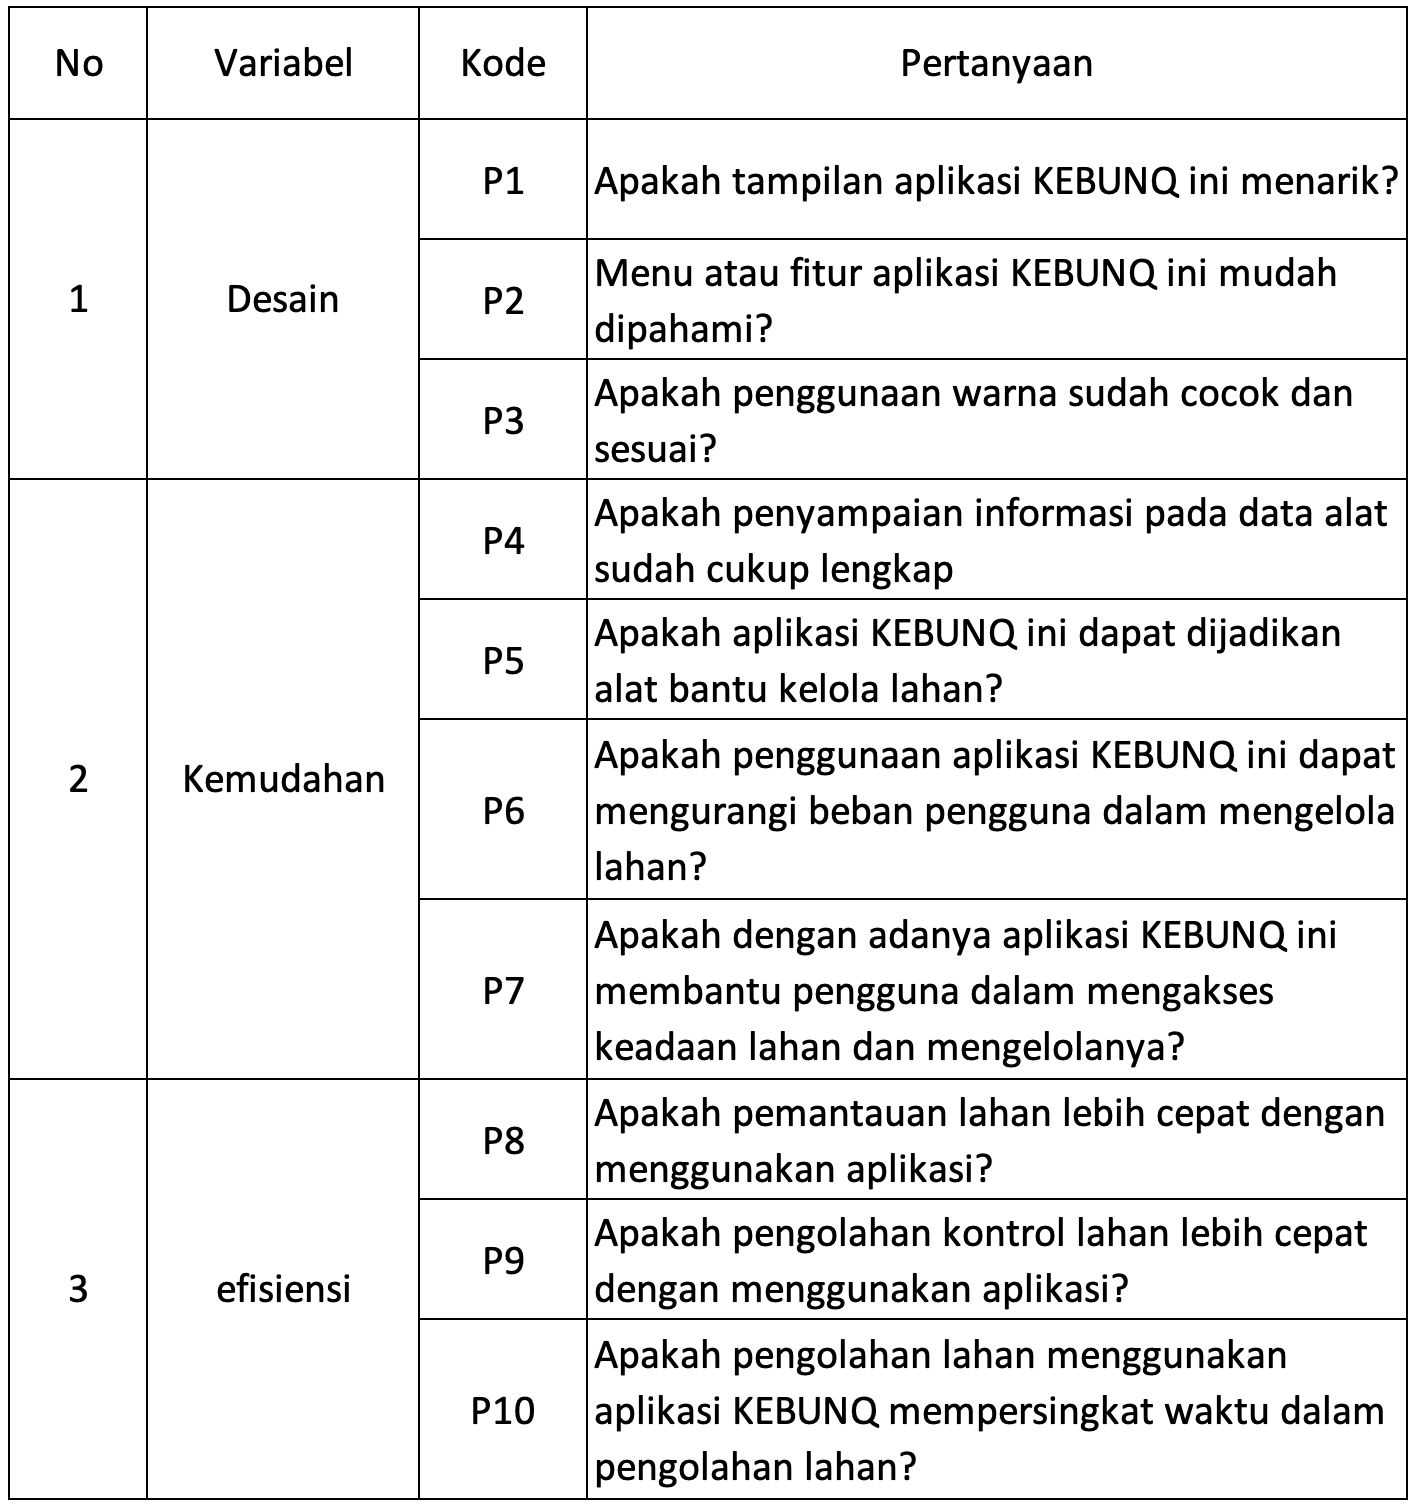
\includegraphics[width=12cm]{images/bab 4/uat.png}\\
            \end{table}
            \vspace{10cm}
       \newline \noindent Hasil kuesioner yang didapat kemudian dihitung jumlahnya berdasarkan setiap jawaban, perhitungan dapat dilihat pada tabel 4.4, berikut:\\
        \begin{table}[ht]
            \centering
            \caption{Jumlah Hasil Kuesioner}
            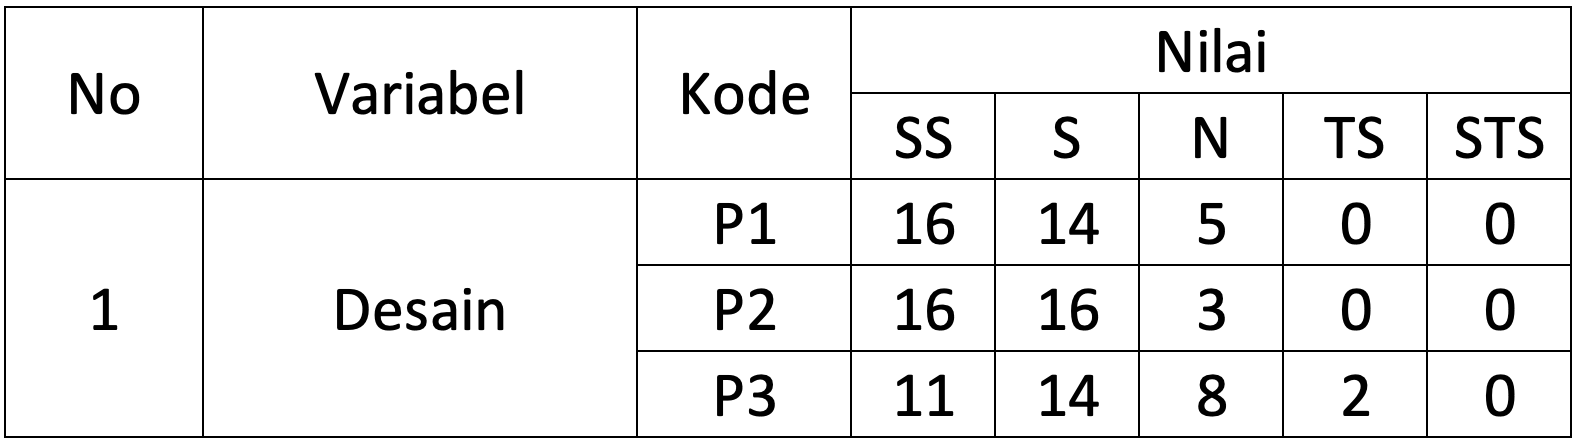
\includegraphics[width=12cm]{images/bab 4/hitungan1-fix.png}\\
            \end{table}
        \begin{table}[ht]
            \centering
            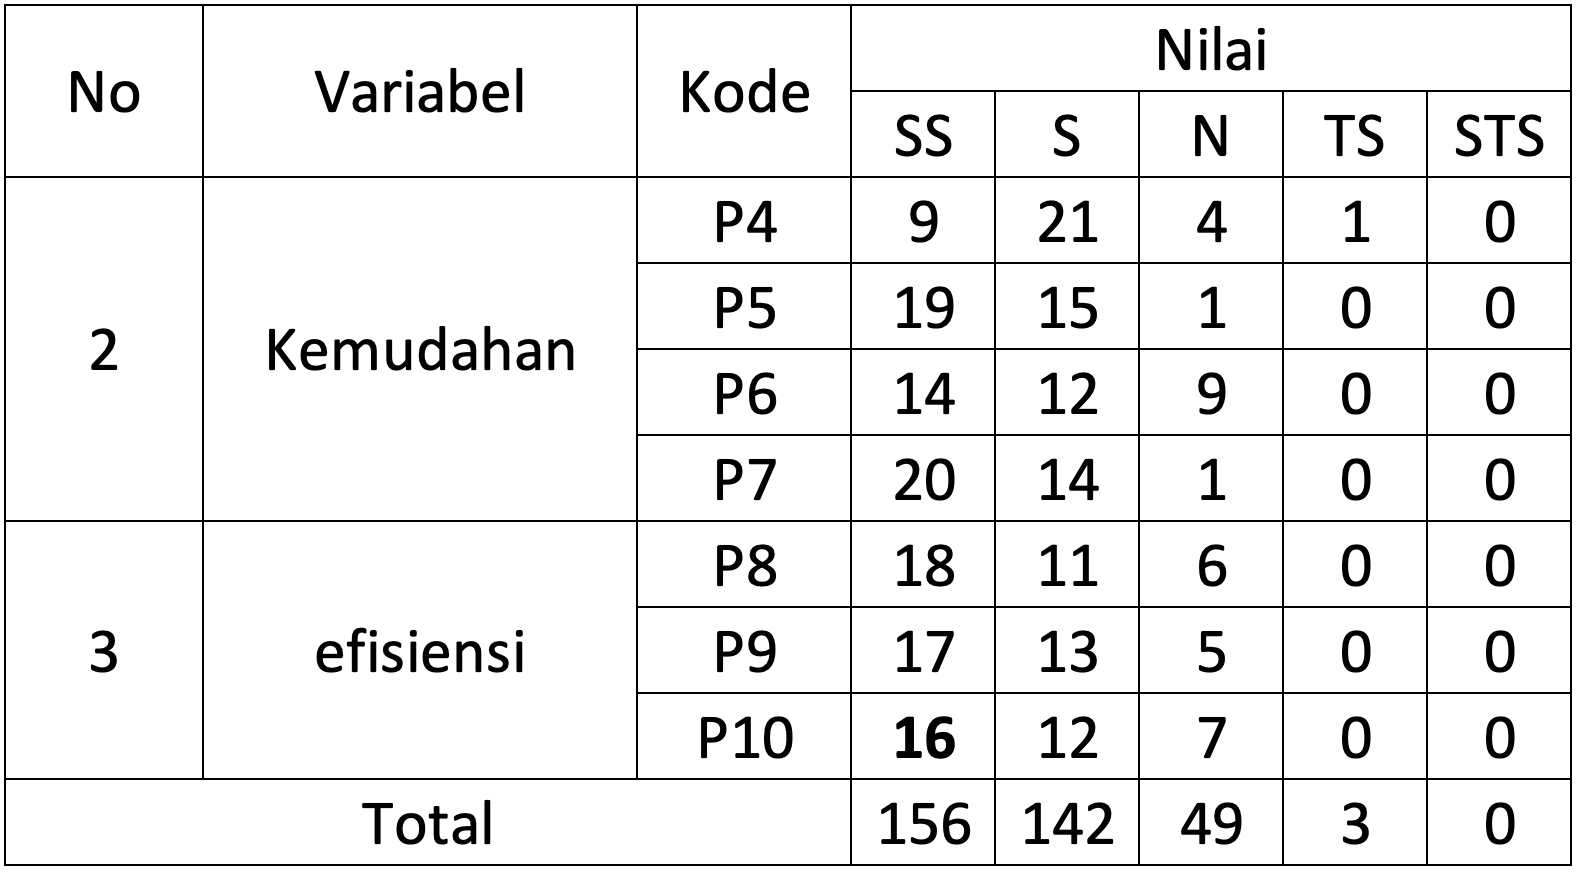
\includegraphics[width=12cm]{images/bab 4/hitungan2-fix.png}\\
            \end{table}
            \vspace{8cm}
            
            \noindent \\Dari data tertera pada Tabel 4.4, dilakukan perhitungan dengan pemberian bobot pada total setiap jawaban.
            Perhitungan pembobotan dapat dilihat sebagai berikut:
            \begin{itemize}
                \item Jumlah skor responden Sangat Setuju (SS) = 156 x 5 = \textbf{780}
                \item Jumlah skor responden Setuju (S)  = 142 x 4 = \textbf{568}
                \item Jumlah skor responden Netral (N)  = 49 x 3 = \textbf{147}
                \item Jumlah skor responden Tidak Setuju (TS)  = 3 x 2 = \textbf{6}
                \item Jumlah skor responden Sangat Tidak Setuju (STS)  = 0 x 1 = \textbf{0}
            \end{itemize}
            Maka didapat jumlah total dari pemberian bobot adalah \textbf{1.501}\\
            Hasil jawaban dari 35 responden tersebut kemudian dilakukan perhitungan nilai terendah dan tertinggi seperti berikut:
            \begin{itemize}
                \item Nilai terendah = 35 x 10 x 1 = \textbf{350}
                \item Nilai tertinggi = 35 x 10 x 5 = \textbf{1.750}
             \end{itemize}
             Hasil perhitungan nilai tertinggi yang didapat adalah 1.750. Kemudian dilakukan perhitungan persentase menggunaan persamaan sebelumnya, sebagai berikut:
             \begin{equation}
                P = \frac{1501}{1750} \times 100\% = 85,77\%
             \end{equation}
             Berdasarkan perhitungan di atas, didapatkan bahwa tingkat penerimaan terhadap aplikasi KEBUNQ terletak pada rentang 81\% - 100\%, 
             masuk dalam kategori nilai kesimpulan sangat kuat sesuai dengan yang dikemukakan oleh Riduwan dalam referensi \cite{kuantitatif}, dengan nilai perhitungan persentase
             85,77\%, yang berarti aplikasi KEBUNQ ini dapat diterima oleh pengguna. Hasil persentase tersebut dapat dilihat pada skala penilaian pada Gambar 4.20 berikut ini:
             \begin{figure}[ht]
                \centering
                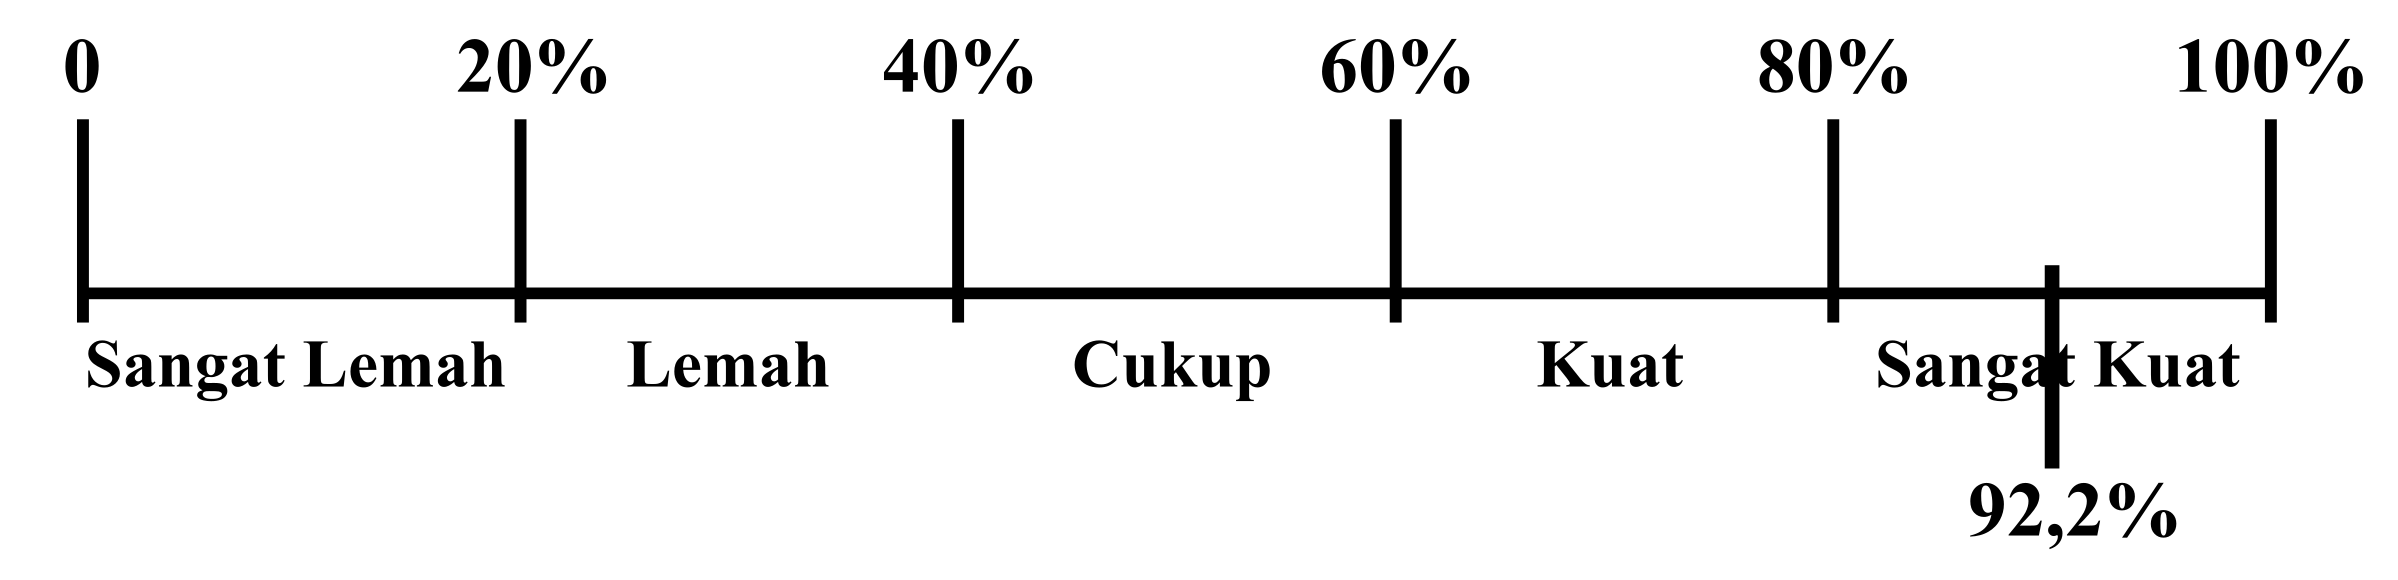
\includegraphics[width=11cm]{images/bab 4/persentase.png}
                \caption{Skala penilaian}
            \end{figure}


   
        \section{Pembahasan}
        Pada tahap observasi didapatkan jenis-jenis sensor dan kontrol yang akan dimasukkan pada penentuan 
        bagaimana aplikasi dirancang dan dibuat menjadi sedinamis mungkin sehingga aplikasi dapat dengan mudah 
        menampilkan sensor dan kontrol dari alat-alat yang debuat berbeda antara alat satu dengan lainnya. 
        Pada tahap pembuatan aplikasi KEBUNQ, peneliti menggunakan \emph{framework Flutter} dengan bahasa 
        pemrograman \emph{Dart}. Dalam penelitian ini dilakukan dua metode pengujian yaitu \emph{black box testing} 
        dan UAT. Pada pengujian \emph{black box} semua hasil menunjukkan kesesuaian dengan apa yang diharapkan, 
        sedangkan pada pengujian UAT yang melibatkan 35 responden, didapatkan hasil persentase sebesar 85,77\% yang 
        menunjukkan penerimaan pengguna yang sangat kuat.
         

    








    \end{justify}




    
\end{flushleft}

\newpage